%=======================================================================
% riscv-privileged.tex
%-----------------------------------------------------------------------

\documentclass[twoside,11pt]{book}
\setcounter{tocdepth}{4}
\setcounter{secnumdepth}{4}

% Package includes

\usepackage{graphicx}
\usepackage{geometry}
\usepackage{array}
\usepackage{colortbl}
\usepackage[colorlinks=true,linkcolor=blue]{hyperref}
\usepackage{placeins}
\usepackage{bbding}
\usepackage{longtable}
\usepackage{multirow}
\usepackage{float}

\usepackage{tabulary}
\usepackage{listings}
\usepackage{algorithmicx}
\usepackage{program}
\usepackage[nochapter]{vhistory}
\usepackage{float}
% If LaTeX just doesn't do what I want, buy http://www.amazon.com/gp/product/0201362996

% Used for tables that can span pages:
\usepackage{xtab}

% Keep spacing normal in enumerated instead of adding extra space between
% items.
\usepackage{enumitem}
%\setlist{nolistsep}

\newenvironment{steps}[1]
  {
     \vspace{1ex}
     \noindent #1
     \begin{enumerate}[nolistsep]
  }
  {
     \end{enumerate}
     \vspace{1ex}
 }

% Setup margins

\setlength{\topmargin}{-0.5in}
\setlength{\textheight}{9in}
\setlength{\oddsidemargin}{0in}
\setlength{\evensidemargin}{0in}
\setlength{\textwidth}{6.5in}

% Useful macros

\newcommand{\note}[1]{{\bf [ NOTE: #1 ]}}
\newcommand{\fixme}[1]{{\bf [ FIXME: #1 ]}}
\newcommand{\todo}[1]{\marginpar{\footnotesize #1}}

\newcommand{\wunits}[2]{\mbox{#1\,#2}}
\newcommand{\um}{\mbox{$\mu$m}}
\newcommand{\xum}[1]{\wunits{#1}{\um}}
\newcommand{\by}[2]{\mbox{#1$\times$#2}}
\newcommand{\byby}[3]{\mbox{#1$\times$#2$\times$#3}}

\newlength\savedwidth
\newcommand\whline[1]{%
  \noalign{%
    \global\savedwidth\arrayrulewidth\global\arrayrulewidth 1.5pt%
  }%
  \cline{#1}%
  \noalign{\vskip\arrayrulewidth}%
  \noalign{\global\arrayrulewidth\savedwidth}%
}

% Custom list environments

\newenvironment{commentary}
{ \vspace{-0.2in}
  \begin{quotation}
  \noindent
  \small \em
  \rule{\linewidth}{1pt}\\
}
{ 
  \end{quotation}
  \vspace{-0.2in}
}

% Other commands and parameters

\pagestyle{myheadings}
\setlength{\parindent}{0in}
\setlength{\parskip}{10pt}
\sloppy

% Commands for register format figures.

% New column types to use in tabular environment for instruction formats.
% Allocate 0.18in per bit.
\newcolumntype{I}{>{\centering\arraybackslash}p{0.18in}}
% Two-bit centered column.
\newcolumntype{W}{>{\centering\arraybackslash}p{0.36in}}
% Three-bit centered column.
\newcolumntype{F}{>{\centering\arraybackslash}p{0.54in}}
% Four-bit centered column.
\newcolumntype{Y}{>{\centering\arraybackslash}p{0.72in}}
% Five-bit centered column.
\newcolumntype{R}{>{\centering\arraybackslash}p{0.9in}}
% Six-bit centered column.
\newcolumntype{S}{>{\centering\arraybackslash}p{1.08in}}
% Seven-bit centered column.
\newcolumntype{O}{>{\centering\arraybackslash}p{1.26in}}
% Eight-bit centered column.
\newcolumntype{E}{>{\centering\arraybackslash}p{1.44in}}
% Ten-bit centered column.
\newcolumntype{T}{>{\centering\arraybackslash}p{1.8in}}
% Twelve-bit centered column.
\newcolumntype{M}{>{\centering\arraybackslash}p{2.2in}}
% Sixteen-bit centered column.
\newcolumntype{K}{>{\centering\arraybackslash}p{2.88in}}
% Twenty-bit centered column.
\newcolumntype{U}{>{\centering\arraybackslash}p{3.6in}}
% Twenty-bit centered column.
\newcolumntype{L}{>{\centering\arraybackslash}p{3.6in}}
% Twenty-five-bit centered column.
\newcolumntype{J}{>{\centering\arraybackslash}p{4.5in}}

\newcommand{\instbit}[1]{\mbox{\scriptsize #1}}
\newcommand{\instbitrange}[2]{~\instbit{#1} \hfill \instbit{#2}~}
\newcommand{\reglabel}[1]{\hfill {\tt #1}\hfill\ }

\newcommand{\wiri}{\textbf{WIRI}}
\newcommand{\wpri}{\textbf{WPRI}}
\newcommand{\wlrl}{\textbf{WLRL}}
\newcommand{\warl}{\textbf{WARL}}

\newcommand{\unspecified}{\textsc{unspecified}}


% All registers are named here. That way when we rename one we'll get errors if
% there are still references to the old name.

\usepackage{makeidx}
\makeindex

\usepackage{xspace}
\newcommand{\defregname}[2]{\providecommand{#1}{{\tt #2}\xspace}}
\newcommand{\deffieldname}[2]{\providecommand{#1}{{$|#2|$}\xspace}}
\deffieldname{\Fmprv}{mprv}
\defregname{\Rmstatus}{mstatus}

\defregname{\Azero}{a0}
\defregname{\Aone}{a1}

\defregname{\Rzero}{zero}
\defregname{\Szero}{s0}
\defregname{\Sone}{s1}

\defregname{\Tzero}{t0}

\defregname{\Xzero}{x0}
\defregname{\Xone}{x1}
\defregname{\Xeight}{x8}
\defregname{\Xnine}{x9}
\defregname{\Xten}{x10}
\defregname{\Xeleven}{x11}
\defregname{\Xthirtyone}{x31}
\defregname{\Fone}{f1}
\defregname{\Rpc}{pc}
\defregname{\Rmhartid}{mhartid}
\defregname{\Rmepc}{mepc}
\defregname{\Rdataone}{data1}

\input{hwbp_registers.tex.inc}
\input{core_registers.tex.inc}
\input{jtag_registers.tex.inc}
\input{dm_registers.tex.inc}
\input{sample_registers.tex.inc}
\input{abstract_commands.tex.inc}
\input{sw_registers.tex.inc}

\deffieldname{\Fhartsel}{\hyperref[hartsel]{hartsel}}

\input{vc.tex}

\newcommand{\versionnum}{0.13-DRAFT}


\begin{document}

\title{RISC-V External Debug Support\\
Version \versionnum\\
\GITHash
}
\author{Tim Newsome \textless tim@sifive.com\textgreater}
\date{\GITAuthorDate}
\maketitle

\markboth{RISC-V External Debug Support Version \versionnum}
{RISC-V External Debug Support Version \versionnum}
\thispagestyle{empty}

\frontmatter

\chapter{Preface}

{\bf Warning! This draft specification will change before being accepted as
standard, so implementations made to this draft specification will likely not
conform to the future standard.}


\section*{Acknowledgments}

I would like to thank the following people for their time, feedback, and ideas:
Bruce Ableidinger,
Krste Asanovic,
Allen Baum,
Mark Beal,
Alex Bradbury,
Zhong-Ho Chen,
Monte Dalrymple,
Vyacheslav Dyachenko,
Peter Egold,
Richard Herveille,
Po-wei Huang,
Scott Johnson,
Aram Nahidipour,
Rishiyur Nikhil,
Gajinder Panesar,
Klaus Kruse Pedersen,
Antony Pavlov,
Ken Pettit,
Wesley Terpstra,
Megan Wachs,
Stefan Wallentowitz,
Ray Van De Walker,
Andrew Waterman,
Thomas Wicki,
and Andy Wright.


\tableofcontents
\listoffigures
\listoftables

\mainmatter

\newpage

\chapter{Introduction}
\label{sec:intro}

When a design progresses from simulation to hardware implementation, a user's
control and understanding of the system's current state drops dramatically.
To help bring up and debug low level software and hardware,
it is critical to have good debugging support built into the hardware.
When a robust OS is running on a core, software can handle many
debugging tasks. However, in many scenarios, hardware support is essential.

This document outlines a standard architecture for external debug support
on RISC-V platforms. This architecture allows a variety of implementations and
tradeoffs, which is complementary to the wide range of RISC-V implementations.
At the same time, this specification defines common interfaces to
allow debugging tools and components to target a variety of platforms based on the RISC-V ISA.

System designers may choose to add additional hardware debug support,
but this specification defines a standard interface for common
functionality.

\section{Terminology}

A \emph{platform} is a single integrated circuit consisting of one or more
\emph{components}. Some components may be RISC-V cores, while others may have a different
function. Typically they will all be connected to a single system bus.
A single RISC-V core contains one or more hardware threads, called
\emph{harts}.

\emph{DXLEN} of a hart is its widest supported XLEN, ignoring the current value
of \Fmxl in \Rmisa.

\subsection{Context}

\begin{steps}{This document is written to work with:}
\item The RISC-V Instruction Set Manual, Volume I: User-Level ISA, Document
    Version 2.2 (the ISA Spec)
\item The RISC-V Instruction Set Manual, Volume II: Privileged Architecture,
    Version 1.10 (the Privileged Spec)
\end{steps}

\subsection{Versions}

Version 0.13 of this document was ratified by the RISC-V Foundation's board.
Versions 0.13.$x$ are bug fix releases to that ratified specification.

Version 0.14 will be forwards and backwards compatible with Version 0.13.

\section{About This Document}

\subsection{Structure}

This document contains two parts. The main part of the document is the
specification, which is given in the numbered sections. The second part
of the document is a set of  appendices. The information
in the appendices is intended to clarify and provide examples, but is
not part of the actual specification.

\subsection{Register Definition Format}

All register definitions in this document follow the format shown below.  A
simple graphic shows which fields are in the register. The upper and lower bit
indices are shown to the top left and top right of each field. The total number
of bits in the field are shown below it.

After the graphic follows a table which for each field lists its name,
description, allowed accesses, and reset value. The allowed accesses are listed
in Table~\ref{tab:access}. The reset value is either a constant or ``Preset.''
The latter means it is an implementation-specific legal value.

Names of registers and their fields are hyperlinks to their definition, and are
also listed in the index on page \pageref{index}.

\input{sample_registers.tex}

\begin{table}[htp]
    \centering
    \caption{Register Access Abbreviations}
    \label{tab:access}
    \begin{tabulary}{\textwidth}{|l|L|}
        \hline
        R & Read-only. \\
        \hline
        R/W & Read/Write. \\
        \hline
        R/W1C & Read/Write. For each bit in the field, writing 1 clears that bit. Writing 0 has no effect. \\
        \hline
        WARZ & Write any, read zero. A debugger may write any value. When read
        this field returns 0. \\
        \hline
        W1 & Write-only. Only writing 1 has an effect. When read the returned
        value should be 0. \\
        \hline
        WARL & Write any, read legal. A debugger may write any value. If a
        value is unsupported, the implementation converts the value to one that
        is supported. \\
        \hline
    \end{tabulary}
\end{table}

%\input{reading_order.tex}

\section{Background}

There are several use cases for dedicated debugging hardware, both
internal to a CPU core and with an external connection.
This specification addresses the use cases listed below. Implementations
can choose not to implement every feature, which means some use cases might
not be supported.

\begin{itemize}

\item Debugging low-level software in the absence of an OS or other software.

\item Debugging issues in the OS itself.

\item Bootstrapping a system to test, configure, and program components before
  there is any executable code path in the system.

\item Accessing hardware on a system without a working CPU.

\end{itemize}

In addition, even without a hardware debugging interface,
architectural support in a RISC-V CPU can aid software debugging and
performance analysis by allowing hardware triggers and breakpoints.

\section{Supported Features}

The debug interface described in this specification supports the following features:

\begin{enumerate}
   \item All hart registers (including CSRs) can be read/written.
   \item Memory can be accessed either from the hart's point of view, through
       the system bus directly, or both.
   \item RV32, RV64, and future RV128 are all supported.
   \item Any hart in the platform can be independently debugged.
   \item A debugger can discover almost\footnote{Notable exceptions include
       information about the memory map and peripherals.} everything it needs
       to know itself, without user configuration.
   \item Each hart can be debugged from the very first instruction executed.
   \item A RISC-V hart can be halted when a software breakpoint instruction is
       executed.
   \item Hardware single-step can execute one instruction at a time.
   \item Debug functionality is independent of the debug transport used.
   \item The debugger does not need to know anything about the microarchitecture
       of the harts it is debugging.

   \item Arbitrary subsets of harts can be halted and resumed simultaneously.
       (Optional)
   \item Arbitrary instructions can be executed on
       a halted hart. That means no new debug functionality is needed when a
       core has additional or custom instructions or state, as
       long as there exist programs
       that can move that state into GPRs. (Optional)
   \item Registers can be accessed without halting. (Optional)
   \item A running hart can be directed to execute a short sequence
       of instructions, with little overhead. (Optional)
   \item A system bus master allows memory access without
       involving any hart. (Optional)
   \item A RISC-V hart can be halted when a trigger matches the PC,
       read/write address/data, or an instruction opcode. (Optional)
    \item Harts can be grouped, and harts in the same group will all halt when
        any of them halts. These groups can also react to or notify external
        triggers. (Optional)
\end{enumerate}

This document does not suggest a strategy or implementation for hardware test,
debugging or error detection techniqes. Scan, BIST, etc. are out of scope of
this specification, but this specification does not intend to limit their use
in RISC-V systems.

It is possible to debug code that uses software threads, but there is no
special debug support for it.

\chapter{System Overview} \label{overview}

Figure~\ref{fig:overview} shows the main components of External Debug Support.
Blocks shown in dotted lines are optional. 

\begin{figure}
   \centering
   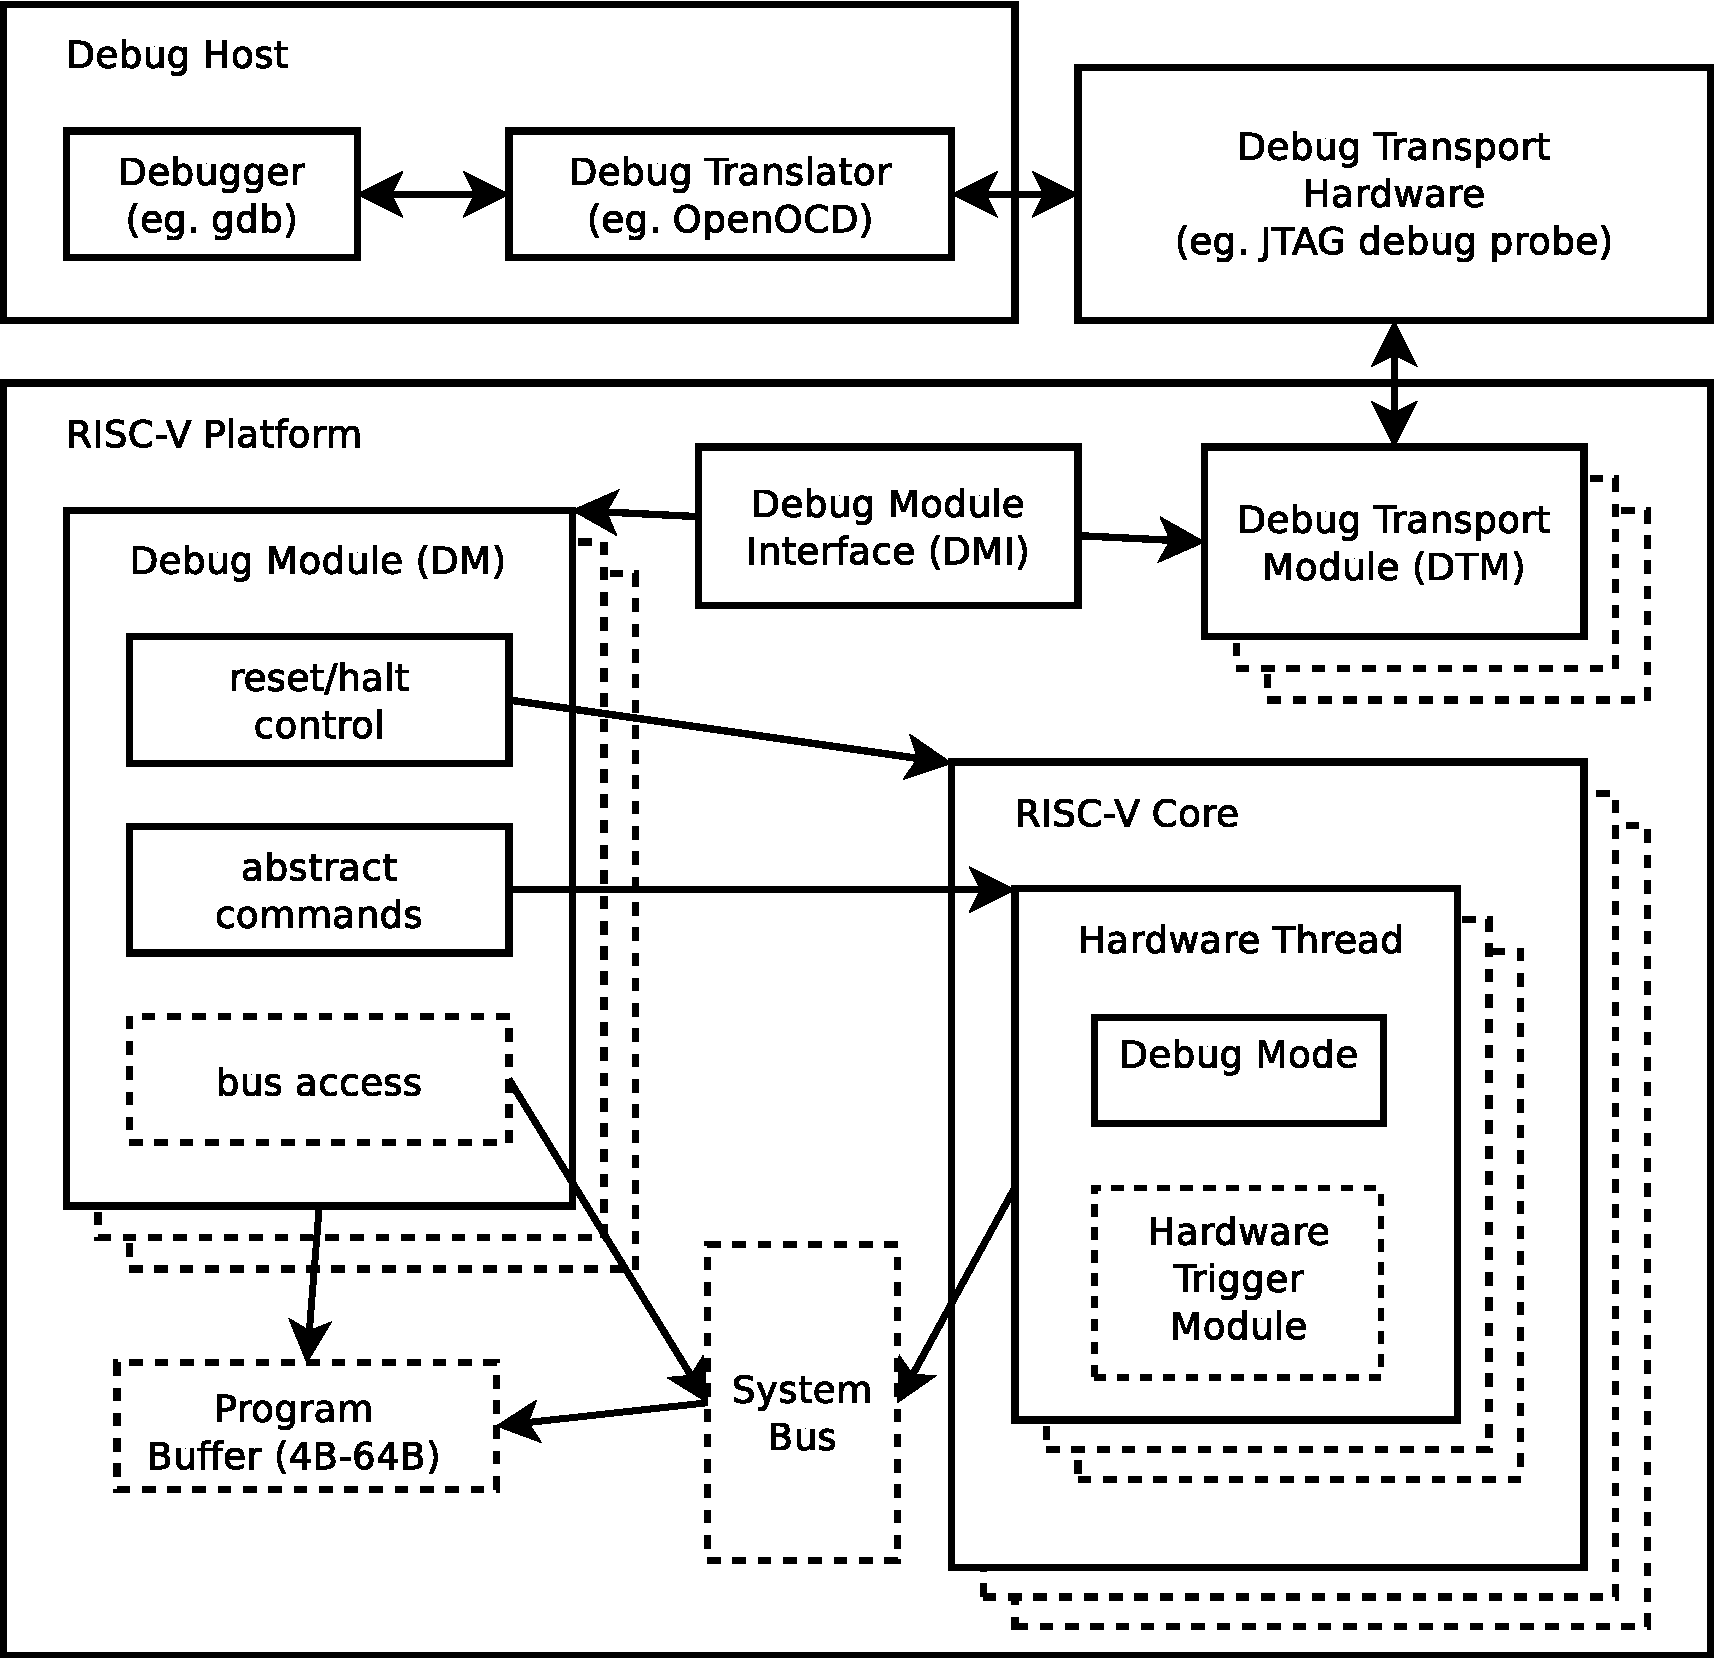
\includegraphics[width=\textwidth]{fig/overview-eps-converted-to.pdf}
   \caption{RISC-V Debug System Overview}
   \label{fig:overview}
\end{figure}

The user interacts with the Debug Host (e.g.\ laptop), which is running a
debugger (e.g.\ gdb).  The debugger communicates with a Debug Translator (e.g.\ 
OpenOCD, which may include a hardware driver) to communicate with Debug
Transport Hardware (e.g.\ Olimex USB-JTAG adapter).
The Debug Transport Hardware connects the Debug Host to the Platform's Debug
Transport Module (DTM).  The DTM provides access to one or more Debug Modules
(DMs) using the Debug Module Interface (DMI).

Each hart in the platform is controlled by exactly one DM. Harts may be
heterogeneous. There is no further limit on the hart-DM mapping, but usually
all harts in a single core are controlled by the same DM. In most platforms there
will only be one DM that controls all the harts in the platform.

DMs provide run control of their harts in the platform. Abstract commands
provide access to GPRs. Additional registers are accessible through abstract
commands or by writing programs to the optional Program Buffer.

The Program Buffer allows the debugger to execute arbitrary instructions on a
hart. This mechanism can also be used to access memory.  An optional system bus
access block allows memory accesses without using a RISC-V hart to perform the
access.

Each RISC-V hart may implement a Trigger Module. When trigger conditions
are met, harts will halt and inform the debug module that they have
halted.

\chapter{Debug Module (DM)} \label{dm}

\begin{steps}{The Debug Module implements a translation interface between abstract debug
    operations and their specific implementation. It might support the following
    operations:}
\item Give the debugger necessary information about the implementation. (Required)
\item Allow any individual hart to be halted and resumed. (Required)
\item Provide status on which harts are halted. (Required)
\item Provide abstract read and write access to a halted hart's GPRs. (Required)
\item Provide access to a reset signal that allows debugging from the very
    first instruction after reset. (Required)
\item Provide a mechanism to allow debugging harts immediately out of reset
      (regardless of the reset cause). (Optional)
\item Provide abstract access to non-GPR hart registers. (Optional)
\item Provide a Program Buffer to force the hart to execute arbitrary instructions. (Optional)
\item Allow multiple harts to be halted, resumed, and/or reset at the same time. (Optional)
\item Allow memory access from a hart's point of view. (Optional)
\item Allow direct System Bus Access. (Optional)
\item Group harts. When any hart in the group halts, they all halt. (Optional)
\item Respond to external triggers by halting each hart in a configured group. (Optional)
\item Signal an external trigger when a hart in a group halts. (Optional)
\end{steps}

\begin{steps}{In order to be compliant with this specification an
    implementation must:}
\item Implement all the required features listed above.
\item Implement at least one of Program Buffer, System Bus Access, or Abstract
    Access Memory command mechanisms.
\item
    \begin{steps}{Do at least one of:}
        \item Implement the Program Buffer.
        \item Implement abstract access to all registers that are visible to
            software running on the hart including all the registers that are
            present on the hart and listed in Table~\ref{tab:regno}.
        \item Implement abstract access to at least all GPRs, \RcsrDcsr, and
            \RcsrDpc, and advertise the implementation as conforming to the
            ``Minimal RISC-V Debug Specification \versionnum'', instead of the
            ``RISC-V Debug Specification \versionnum''.
    \end{steps}
\end{steps}

A single DM can debug up to $2^{20}$ harts.

\section{Debug Module Interface (DMI)} \label{dmi}

Debug Modules are slaves to a bus called the Debug Module Interface (DMI). The
master of the bus is the Debug Transport Module(s).
The Debug Module Interface can be a trivial bus with one master and one slave,
or use a more full-featured bus like TileLink or the AMBA Advanced Peripheral
Bus. The details are left to the system designer.

The DMI uses between 7 and 32 address bits.  It supports read and write
operations.  The bottom of the address space is
used for the first (and usually only) DM. Extra space can be used for custom
debug devices, other cores, additional DMs, etc. If there are additional DMs
on this DMI, the base address of the next DM in the DMI address space is given
in \RdmNextdm.

The Debug Module is controlled via register accesses to its DMI address space.

\section{Reset Control} \label{reset}

There are two methods that allow a debugger to reset harts.
\FdmDmcontrolNdmreset resets all the harts in the system, as well as all other
parts of the system except for the Debug Modules, Debug Transport Modules,
and Debug Module Interface.
Exactly what is affected by this reset is implementation dependent, but it
must be possible to debug programs from the first instruction executed.
\FdmDmcontrolHartreset resets all the currently selected harts. In this case an
implementation may reset more harts than just the ones that are selected. The
debugger can discover which other harts are reset (if any) by selecting them
and checking \FdmDmstatusAnyhavereset and \FdmDmstatusAllhavereset.

To perform either of these resets, the debugger first asserts the bit, and then
clears it. The actual reset may start as soon as the bit is asserted, but may
start an arbitrarily long time after the bit is deasserted. The reset itself
may also take an arbitrarily long time.  While the reset is
on-going, harts are either in the running state, indicating it's possible to
perform some abstract commands during this time, or in the unavailable state,
indicating it's not possible to perform any abstract commands during this time.
Once a hart's reset is complete, {\tt havereset} becomes set.  When a hart comes out
of reset and \FdmDmcontrolHaltreq or \Fresethaltreq are set, the hart will
immediately enter Debug Mode (halted state). Otherwise it will execute normally
(running state).

\begin{commentary}
    There is no general, reliable way for the debugger to know when reset has
    actually begun.
\end{commentary}

The halt state of harts should be
maintained across system reset provided that \FdmDmcontrolDmactive is 1,
although trigger CSRs may be cleared.

The Debug Module's own state and registers should only be
reset at power-up and while
\FdmDmcontrolDmactive in \RdmDmcontrol is 0. If there is another mechanism to
reset the DM, this mechanism must also reset all the harts accessible to the
DM.

Due to clock and power domain crossing issues,
it may not be possible to perform arbitrary DMI accesses across
system reset.
While \FdmDmcontrolNdmreset or any external reset is asserted, the only supported DM
operations are reading and writing \RdmDmcontrol. The behavior of other accesses
is undefined.

When harts have been reset, they must set a sticky {\tt havereset} state bit.
The conceptual {\tt havereset} state bits can be read for selected harts in
\FdmDmstatusAnyhavereset and \FdmDmstatusAllhavereset in \RdmDmstatus.
These bits must be set regardless of the cause of the reset.
The {\tt havereset} bits for the selected harts
can be cleared by writing 1 to \FdmDmcontrolAckhavereset in \RdmDmcontrol.
The {\tt havereset} bits may or may not be cleared
when \FdmDmcontrolDmactive is low.

\section{Selecting Harts} \label{selectingharts}

Up to $2^{20}$ harts can be connected to a single DM. The debugger
selects a hart, and then subsequent halt, resume, reset, and debugging
commands are specific to that hart.

To enumerate all the harts, a debugger must first determine {\tt HARTSELLEN}
by writing  all ones to \Fhartsel (assuming the maximum size) and reading back
the value to see which bits were actually set.  Then it selects each hart
starting from 0 until either \FdmDmstatusAnynonexistent in \RdmDmstatus is 1, or the
highest index (depending on {\tt HARTSELLEN}) is reached.

The debugger can discover the mapping between hart indices and
\Rmhartid by using the interface to read \Rmhartid, or by
reading the system's configuration string.

\subsection {Selecting a Single Hart}

All debug modules must support selecting a single hart.
The debugger can select a hart by writing its index to \Fhartsel.
Hart indexes start at 0 and are contiguous until the final index.

\subsection {Selecting Multiple Harts} \label{hartarraymask}

Debug Modules may implement a Hart Array Mask register to allow selecting
multiple harts at once. The $n$th bit in the Hart Array Mask register applies to
the hart with index $n$. If the bit is 1 then the hart is selected.  Usually a DM
will have a Hart Array Mask register exactly wide enough to select all the
harts it supports, but it's allowed to tie any of these bits to 0.

The debugger can set bits in the hart array mask register using \RdmHawindowsel
and \RdmHawindow, then apply actions to all selected harts by setting \FdmDmcontrolHasel. If
this feature is supported, multiple harts can be halted, resumed, and reset
simultaneously. The state of the hart array mask register is not affected by
setting or clearing \FdmDmcontrolHasel.

Only the actions initiated by \RdmDmcontrol can apply to multiple harts
at once, Abstract Commands apply only to the hart selected by
\Fhartsel.

\section{Hart DM States}

Every hart that can be selected is in exactly one of the following four DM states:
non-existent, unavailable, running, or halted. Which state
the selected harts are in is reflected by \FdmDmstatusAllnonexistent,
\FdmDmstatusAnynonexistent, \FdmDmstatusAllunavail, \FdmDmstatusAnyunavail,
\FdmDmstatusAllrunning, \FdmDmstatusAnyrunning, \FdmDmstatusAllhalted, and
\FdmDmstatusAnyhalted.

Harts are nonexistent if they will never be part of this system, no matter how
long a user waits. E.g.\ in a simple single-hart system only one hart exists,
and all others are nonexistent. Debuggers may assume that a system has no harts
with indexes higher than the first nonexistent one.

Harts are unavailable if they might exist/become available at a later time, or
if there are other harts with higher indexes than this one. Harts may be
unavailable for a variety of reasons including being reset, temporarily powered
down, and not being plugged into the system.
Systems with very large number of harts may
permanently disable some during manufacturing, leaving holes in the otherwise
continuous hart index space. In order to let the debugger discover all harts,
they must show up as unavailable even if there is no chance of them ever
becoming available.

Harts are running when they are executing normally, as if no debugger was
attached. This includes being in a low power mode or waiting for an interrupt,
as long as a halt request will result in the hart being halted.

Harts are halted when they are in Debug Mode, only performing tasks on behalf
of the debugger.

Which states a hart that is reset goes through is implementation dependent.
Harts may be unavailable while reset is asserted, and some time after reset is
deasserted. They might transition to running for some time after reset is
deasserted. Finally they end up either running or halted, depending on
\FdmDmcontrolHaltreq and \Fresethaltreq.

\section{Run Control} \label{runcontrol}

For every hart, the Debug Module tracks 4 conceptual bits of state: halt
request, resume ack, halt-on-reset request,  and hart reset.
(The hart reset and halt-on-reset request bits are optional.)
These 4 bits reset to 0, except for resume ack, which may reset to either 0 or 1.
The DM receives halted, running, and havereset signals from each hart.
The debugger can observe the state of resume ack in \FdmDmstatusAllresumeack and
\FdmDmstatusAnyresumeack, and the state of halted, running, and havereset signals
in \FdmDmstatusAllhalted, \FdmDmstatusAnyhalted, \FdmDmstatusAllrunning, \FdmDmstatusAnyrunning, \FdmDmstatusAllhavereset,
and \FdmDmstatusAnyhavereset. The state of the other bits cannot be observed directly.

When a debugger writes 1 to \FdmDmcontrolHaltreq, each selected hart's halt request bit is
set.
When a running hart, or a hart just coming out of reset, sees its halt request
bit high, it responds by halting, deasserting its running signal, and asserting
its halted signal.
Halted harts ignore their halt request bit.

When a debugger writes 1 to \FdmDmcontrolResumereq, each selected hart's resume ack bit is
cleared and each selected, halted hart is sent a resume request. Harts respond
by resuming, clearing their halted signal, and asserting their running signal.
At the end of this process the resume ack bit is set.  These
status signals of all selected harts are reflected in \FdmDmstatusAllresumeack,
\FdmDmstatusAnyresumeack, \FdmDmstatusAllrunning, and \FdmDmstatusAnyrunning. Resume requests are ignored by
running harts.

When halt or resume is requested, a hart must respond in
less than one second, unless it is unavailable.
(How this is implemented is not further specified. A few
clock cycles will be a more typical latency).

The DM can implement optional halt-on-reset bits for each hart,
which it indicates by setting \FdmDmstatusHasresethaltreq to 1.
This means the DM implements the \FdmDmcontrolSetresethaltreq and \FdmDmcontrolClrresethaltreq bits.
Writing 1 to \FdmDmcontrolSetresethaltreq sets the halt-on-reset request bit for each
selected hart.
When a hart's halt-on-reset request bit is set, the hart will immediately enter
debug mode on the next deassertion of its reset. This is true regardless of
the reset's cause.
The hart's halt-on-reset request bit remains set
until cleared by the debugger writing 1 to \FdmDmcontrolClrresethaltreq
while the hart is selected, or by DM reset.

\section{Halt Groups and External Triggers}

An optional feature allows a debugger to create halt groups. When any hart in a
halt group halts all the other harts in that group will quickly halt, even if
they are currently in the process of resuming. Adding a hart to a halt group
does not automatically halt that hart, even if other harts in the group are
already halted.

It is also possible to add external triggers to a halt group. External triggers
are abstract concepts that can signal the DM and/or receive signals from the
DM.  When an external trigger fires, all harts in its halt group are quickly
halted. When a hart in a halt group halts, the external triggers in the same
halt group are notified.

\begin{commentary}
    External triggers could be used to implement near simultaneous halting of
    all cores in a system, when not all cores are RISC-V cores.
\end{commentary}

Halt group 0 is special, and has none of this behavior. Harts in halt group 0
halt as if halt groups aren't implemented at all.

To near simultaneously resume all harts in a group, the debugger can select all
the harts, and write 1 to \FdmDmcontrolResumereq as described above. An implementation
must guarantee that all harts in the group halt again as soon as one of them
halts, even if that hart halts before all harts have resumed.

\section{Abstract Commands} \label{abstractcommands}

The DM supports a set of abstract commands, most of which
are optional. Depending on the implementation, the debugger may
be able to perform
some abstract commands even when the selected hart is not halted.
Debuggers can only determine which abstract commands
are supported by a given hart in a given state (running, halted, or held in reset) by attempting them
and then looking at \FdmAbstractcsCmderr in \RdmAbstractcs to see if they were successful.
Commands may be supported with some options set, but not with other options
set. If a command has unsupported options set or if bits that are defined as 0
aren't 0, then the DM must set \FdmAbstractcsCmderr to 2 (not supported).

\begin{commentary}
    Example: Every system must support the Access Register command, but may not
    support accessing CSRs. If the debugger requests to read a CSR in that
    case, the command will return ``not supported.''
\end{commentary}

Debuggers execute abstract commands by writing them to \RdmCommand.  They
can determine whether an abstract command is complete by reading \FdmAbstractcsBusy in
\RdmAbstractcs. If the debugger starts a new command while \FdmAbstractcsBusy is set,
\FdmAbstractcsCmderr becomes 1 (busy), the currently executing command still gets to
run to completion, but any error generated by the currently executing command is lost.
After completion, \FdmAbstractcsCmderr indicates whether the command was
successful or not. Commands may fail because a hart is not halted, not running,
unavailable, or because they encounter an error during execution.

If the command takes arguments, the debugger
must write them to the {\tt data} registers before writing to \RdmCommand. If a
command returns results, the Debug Module must ensure they are placed
in the {\tt data} registers before \FdmAbstractcsBusy is cleared.
Which {\tt data} registers are used for the arguments is
described in Table~\ref{tab:datareg}.  In all cases the least-significant word
is placed in the lowest-numbered {\tt data} register. The argument width
depends on the command being executed, and is DXLEN where not explicitly
specified.

\begin{table}[htp]
    \centering
    \caption{Use of Data Registers}
    \label{tab:datareg}
    \begin{tabulary}{\textwidth}{|r|l|l|l|}
        \hline
        Argument Width & arg0/return value & arg1 & arg2 \\
        \hline
        32 & \RdmDataZero & {\tt data1} & {\tt data2} \\
        \hline
        64 & \RdmDataZero, {\tt data1} & {\tt data2}, {\tt data3} & {\tt data4}, {\tt data5} \\
        \hline
        128 & \RdmDataZero--{\tt data3} & {\tt data4}--{\tt data7} & {\tt data8}--{\tt data11} \\
        \hline
    \end{tabulary}
\end{table}

\begin{commentary}
    The Abstract Command interface is designed to allow a debugger to write
    commands as fast as possible, and then later check whether they completed
    without error.  In the common case the debugger will be much slower than
    the target and commands succeed, which allows for maximum throughput. If
    there is a failure, the interface ensures that no commands execute after
    the failing one.  To discover which command failed, the debugger has to
    look at the state of the DM (e.g.\ contents of \RdmDataZero) or hart (e.g.\ 
    contents of a register modified by a Program Buffer program) to determine
    which one failed.
\end{commentary}

Before starting an abstract command, a debugger must ensure that \FdmDmcontrolHaltreq,
\FdmDmcontrolResumereq, and \FdmDmcontrolAckhavereset are all 0.

While an abstract command is executing (\FdmAbstractcsBusy in \RdmAbstractcs is high), a
debugger must not change \Fhartsel, and must not write 1 to \FdmDmcontrolHaltreq,
\FdmDmcontrolResumereq, \FdmDmcontrolAckhavereset, \FdmDmcontrolSetresethaltreq, or \FdmDmcontrolClrresethaltreq.

If an abstract command does not complete in the expected time and appears to be
hung, the debugger can try to reset the hart (using \FdmDmcontrolHartreset or
\FdmDmcontrolNdmreset). If that doesn't clear \FdmAbstractcsBusy, then it
can try resetting the Debug Module (using \FdmDmcontrolDmactive).

If an abstract command is started while the selected hart is unavailable or if
a hart becomes unavailable while executing an abstract command, then the
Debug Module may terminate the abstract command, setting \FdmAbstractcsBusy low, and
\FdmAbstractcsCmderr to 4 (halt/resume). Alternatively, the command could just appear to be
hung (\FdmAbstractcsBusy never goes low).

\subsection{Abstract Command Listing}

This section describes each of the different abstract commands
and how their fields should be interpreted when
they are written to \RdmCommand.

Each abstract command is a 32-bit value. The top 8 bits contain \FdmCommandCmdtype which
determines the kind of command. Table~\ref{tab:cmdtype} lists all commands.

\begin{table}[htp]
    \centering
    \caption{Meaning of \FdmCommandCmdtype}
    \label{tab:cmdtype}
    \begin{tabulary}{\textwidth}{|r|l|l|l|}
        \hline
        \FdmCommandCmdtype & Command & Page \\
        \hline
        0 & Access Register Command & \pageref{acAccessregister} \\
        \hline
        1 & Quick Access & \pageref{acQuickaccess} \\
        \hline
        2 & Access Memory Command & \pageref{acAccessmemory} \\
        \hline
    \end{tabulary}
\end{table}

\input{abstract_commands.tex}

\section{Program Buffer} \label{programbuffer}

To support executing arbitrary instructions on a halted hart,
a Debug Module can include a Program Buffer that a debugger
can write small programs to. Systems
that support all necessary functionality using abstract commands
only may choose to omit the Program Buffer.

A debugger can write a small program to the Program Buffer, and then
execute it exactly once with the Access Register Abstract Command,
setting the \FacAccessregisterPostexec bit in \RdmCommand.
The debugger can write whatever program it likes (including jumps out of the
Program Buffer), but the program must end with
{\tt ebreak} or {\tt c.ebreak}. An implementation may support
an implied {\tt ebreak} that is executed when a hart runs off the end of the
Program Buffer. This is indicated by \FdmDmstatusImpebreak. With this feature, a Program
Buffer of just 2 32-bit words can offer efficient debugging.

If \FdmAbstractcsProgbufsize is 1, \FdmDmstatusImpebreak must be 1. It is possible that the Program
Buffer can hold only one 32- or 16-bit instruction, so the debugger must only
write a single instruction in this case, regardless of its size.
This instruction can be a 32-bit
instruction, or a compressed instruction in the lower 16 bits accompanied by a
compressed {\tt nop} in the upper 16 bits.

\begin{commentary}
    The slightly inconsistent behavior with a Program Buffer of size 1 is to
    accommodate hardware designs that prefer to stuff instructions directly
    into the pipeline when halted, instead of having the Program Buffer exist
    in the address space somewhere.
\end{commentary}

While these programs are executed, the hart does not leave Debug Mode (see
Section~\ref{debugmode}).  If an exception is encountered during execution of
the Program Buffer, no more instructions are executed, the hart remains in Debug
Mode, and \FdmAbstractcsCmderr is set to 3 ({\tt exception error}).  If the debugger
executes a program that doesn't terminate with an {\tt ebreak} instruction, the
hart will remain in Debug Mode and the debugger will lose control of the hart.

Executing the Program Buffer may clobber \RcsrDpc. If that is the case, it must be
possible to read/write \RcsrDpc using an abstract command with \FacAccessregisterPostexec not set.
The debugger must attempt to save \RcsrDpc between halting and
executing a Program Buffer, and then restore \RcsrDpc before leaving Debug Mode.

\begin{commentary}
    Allowing Program Buffer execution to clobber \RcsrDpc allows for direct
    implementations that don't have a separate PC register, and do need to use
    the PC when executing the Program Buffer.
\end{commentary}

The Program Buffer may be implemented as RAM which is accessible to the
hart. A debugger can determine if this is the case by executing small
programs that attempt to write and read back relative to \Rpc while executing
from the Program Buffer.
If so, the debugger has more flexibility in what it can do with the program buffer.

\section{Overview of Hart Debug States}

Figure~\ref{fig:abstract_sm} shows a conceptual view of the states
passed through by a hart during run/halt debugging as influenced
by the different fields of \RdmDmcontrol, \RdmAbstractcs, \RdmAbstractauto, and
\RdmCommand.

\begin{figure}
   \centering
   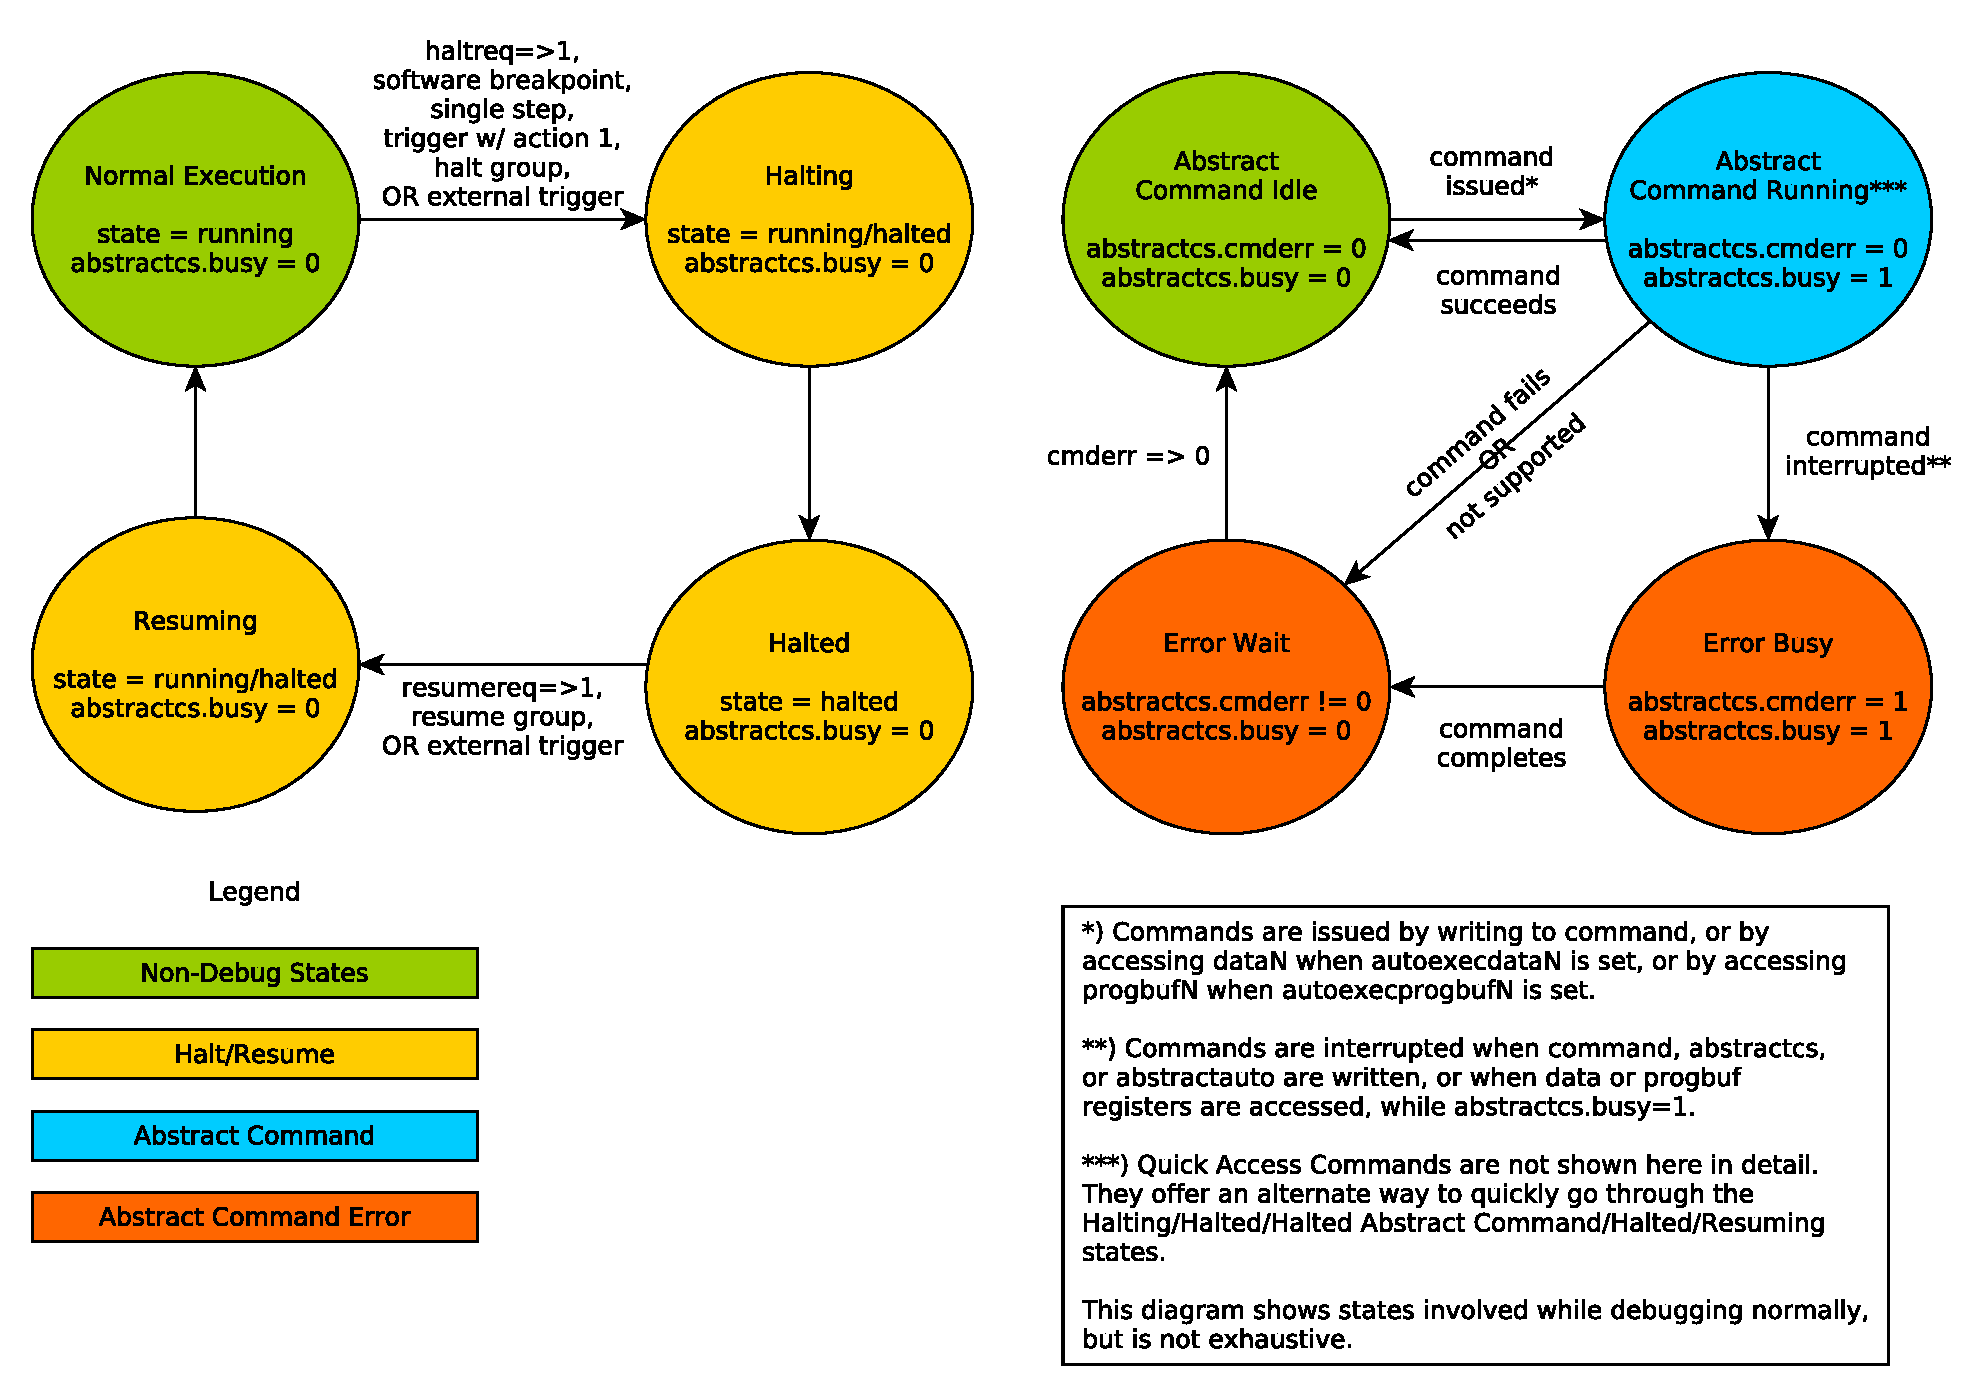
\includegraphics[width=\textwidth]{fig/abstract_commands.pdf}
   \caption[Run/Halt Debug State Machine]{Run/Halt Debug State Machine for single-hart systems.
     As only a small amount of state is visibile to the debugger,
     the states and transitions are conceptual.}
   \label{fig:abstract_sm}
\end{figure}

\section{System Bus Access} \label{systembusaccess}

A debugger can access memory from a hart's point of view using a Program Buffer or
the Abstract Access Memory command. (Both these features are optional.)
A Debug Module may also include a System Bus Access block to provide memory
access without
involving a hart, regardless of whether Program Buffer is implemented.
The System Bus Access block uses physical addresses.

The System Bus Access block may support 8-, 16-, 32-, 64-, and 128-bit
accesses. Table~\ref{tab:sbdatabits} shows which bits in {\tt sbdata} are used
for each access size.

\begin{table}[htp]
    \centering
    \caption{System Bus Data Bits}
    \label{tab:sbdatabits}
    \begin{tabulary}{\textwidth}{|r|l|}
        \hline
        Access Size & Data Bits \\
        \hline
        8 & \RdmSbdataZero bits 7:0 \\
        \hline
        16 & \RdmSbdataZero bits 15:0 \\
        \hline
        32 & \RdmSbdataZero \\
        \hline
        64 & \RdmSbdataOne, \RdmSbdataZero \\
        \hline
        128 & \RdmSbdataThree, \RdmSbdataTwo, \RdmSbdataOne, \RdmSbdataZero \\
        \hline
    \end{tabulary}
\end{table}

Depending on the microarchitecture, data accessed through System Bus Access may
not always be coherent with that observed by each hart. It is up to the
debugger to enforce coherency if the implementation does not. This
specification does not define a standard way to do this.
Possibilities may include
writing to special memory-mapped
locations, or executing special instructions via the Program Buffer.

\begin{commentary}
Implementing a System Bus Access block has several benefits even
when a Debug Module also implements a Program Buffer.
First, it is possible to
access memory in a running system with minimal impact.  Second, it may improve
performance when accessing memory.
Third, it may provide
access to devices that a hart does not have access to.
\end{commentary}

\section{Minimally Intrusive Debugging}

Depending on the task it is performing, some harts can only be halted very briefly.
There are several mechanisms that allow accessing resources in such a running system
with a minimal impact on the running hart.

First, an implementation may allow some abstract commands to execute without halting the hart.

Second, the Quick Access abstract command can be used to halt a hart, quickly
execute the contents of the Program Buffer, and let the hart run again.
Combined with instructions that allow Program Buffer code to access the
{\tt data} registers, as described in \ref{hartinfo}, this can be used to quickly
perform a memory or register access. For some systems this will be too
intrusive, but many systems that can't be halted can bear an occasional hiccup
of a hundred or less cycles.

Third, if the System Bus Access block is implemented, it can be used while a
hart is running to access system memory.

\section{Security}

To protect intellectual property it may be desirable to lock access to the
Debug Module.  To allow access during a manufacturing process and not
afterwards, a reasonable solution could be to add a fuse bit to the Debug
Module that can be used to be permanently disable it. Since this is technology
specific, it is not further addressed in this spec.

Another option is to allow the DM to be unlocked only by users who have an
access key. Between \FdmDmstatusAuthenticated, \FdmDmstatusAuthbusy, and \RdmAuthdata arbitrarily
complex authentication mechanism can be supported.  When \FdmDmstatusAuthenticated is
clear, the DM must not interact with the rest of the platform, nor expose
details about the harts connected to the DM. All DM registers should read 0,
while writes should be ignored, with the following mandatory exceptions:
\begin{steps}{}
    \item \FdmDmstatusAuthenticated in \RdmDmstatus is readable.
    \item \FdmDmstatusAuthbusy in \RdmDmstatus is readable.
    \item \FdmDmstatusVersion in \RdmDmstatus is readable.
    \item \FdmDmcontrolDmactive in \RdmDmcontrol is readable and writable.
    \item \RdmAuthdata is readable and writable.
\end{steps}

\section{Version Detection}

\begin{steps}{To detect the version of the Debug Module with a minimum of side
    effects, use the following procedure:}
    \item Read \RdmDmcontrol.
    \item Write \RdmDmcontrol, preserving \FdmDmcontrolHartreset, \FdmDmcontrolHasel, \FdmDmcontrolHartsello, and
        \FdmDmcontrolHartselhi from the value that was read, setting \FdmDmcontrolDmactive, and
        clearing all the other bits.
    \item Read \RdmDmstatus, which contains \FdmDmstatusVersion.
\end{steps}

\begin{steps}{This has the following unavoidable side effects:}
    \item \FdmDmcontrolHaltreq is cleared, potentially preventing a halt request made by a
        previous debugger from taking effect.
    \item \FdmDmcontrolResumereq is cleared, potentially preventing a resume request made
        by a previous debugger from taking effect.
    \item \FdmDmcontrolNdmreset is deasserted, releasing the system from reset if a
        previous debugger had set it.
    \item \FdmDmcontrolDmactive is asserted, releasing the DM from reset. This in itself
        is not observable by any harts.
\end{steps}

This procedure is guaranteed to work in future versions of this spec.  The
meaning of the \RdmDmcontrol bits where \FdmDmcontrolHartreset, \FdmDmcontrolHasel, \FdmDmcontrolHartsello, and
\FdmDmcontrolHartselhi currently reside might change, but preserving them will have no
side effects. Clearing the bits of \RdmDmcontrol not explicitly mentioned here
will have no side effects beyond the ones mentioned above.

\section{Debug Module Registers} \label{dmdebbus}

The registers described in this section are accessed over the DMI bus.  Each DM
has a base address (which is 0 for the first DM). The register addresses below
are offsets from this base address.

When read, unimplemented Debug Module DMI Registers return 0. Writing them has
no effect.

For each register it is possible to determine that it is implemented by reading
it and getting a non-zero value (e.g.\ \RdmSbcs), or by checking bits in another
register (e.g.\ \FdmAbstractcsProgbufsize).

\input{dm_registers.tex}

\chapter{RISC-V Debug}
\label{sec:core_debug}

Modifications to the RISC-V core to support debug are kept to a minimum.  There
is a special execution mode (Debug Mode) and a few extra CSRs. The DM takes care
of the rest.

\section{Debug Mode} \label{debugmode}

Debug Mode is a special processor mode used only when a hart is halted for
external debugging. How Debug Mode is implemented is not specified here.

\begin{steps}{When executing code from the Program Buffer, the hart stays
    in Debug Mode and the following apply:}
\item All operations are executed at machine mode privilege level, except that
    \Fmprv in \Rmstatus may be ignored according to \Fmprven.
    \begin{commentary}
      In general, the debugger is expected to be able to simulate all the effects of \Fmprv.
      The exception is the case of Sv32 systems, which need \Fmprv functionality in order to access
      34-bit physical addresses. Other systems are likely to tie \Fmprven to 0.
    \end{commentary}
\item All interrupts (including NMI) are masked.
\item Exceptions don't update any registers.  That includes {\tt cause}, {\tt
    epc}, {\tt tval}, {\tt dpc}, and \Rmstatus. They do end execution of the
    Program Buffer.
\item No action is taken if a trigger matches.
\item Trace is disabled.
\item Counters may be stopped, depending on \Fstopcount in \Rdcsr.
\item Timers may be stopped, depending on \Fstoptime in \Rdcsr.
\item The {\tt wfi} instruction acts as a {\tt nop}.
\item Almost all instructions that change the privilege level have undefined
    behavior.  This includes {\tt ecall}, {\tt mret}, {\tt hret}, {\tt sret},
    and {\tt uret}.  (To change the privilege level, the debugger can write
    \Fprv in \Rdcsr). The only exception is {\tt ebreak}. When that is executed
    in Debug Mode, it halts the hart again but without updating \Rdpc or \Rdcsr.
\end{steps}

\section{Load-Reserved/Store-Conditional Instructions}

The reservation registered by an {\tt lr} instruction on a memory address may
be lost when entering Debug Mode or while in Debug Mode.  This means that there
may be no forward progress if Debug Mode is entered between {\tt lr} and {\tt
sc} pairs.

\begin{commentary}
    This is a behavior that debug users must be aware of. If they have a
    breakpoint set between a {\tt lr} and {\tt sc} pair, or are stepping
    through such code, the {\tt sc} may never succeed.  Fortunately in general use
    there will be very few instructions in such a sequence, and anybody
    debugging it will quickly notice that the reservation is not occurring.
    The solution in that case is to set a breakpoint on the first instruction
    after the {\tt sc} and run to it.
\end{commentary}

\section{Single Step}

A debugger can cause a halted hart to execute a single instruction and then
re-enter Debug Mode by setting \Fstep before setting \Fresumereq.

If executing or fetching that instruction causes an exception, Debug Mode is
re-entered immediately after the PC is changed to the exception handler and the
appropriate {\tt tval} and {\tt cause} registers are updated.

If executing or fetching the instruction causes a trigger to fire, Debug Mode
is re-entered immediately after that trigger has fired. In that case \Fcause is
set to 2 (trigger) instead of 4 (single step).  Whether the instruction is
executed or not depends on the specific configuration of the trigger.

If the instruction that is executed causes the PC to change to an address where
an instruction fetch causes an exception, that exception does not occurr until
the next time the hart is resumed. Similarly, a trigger at the new address does
not fire until the hart actually attempts to execute that instruction.

\section{Reset}

If the halt signal (driven by the hart's halt request bit in the Debug Module)
is asserted when a hart comes out of reset, the hart must
enter Debug Mode before executing any instructions, but after performing any
initialization that would usually happen before the first instruction is
executed.

\subsection{{\tt dret} Instruction} \label{dret}

To return from Debug Mode, a new instruction is defined: {\tt dret}. It has an
encoding of 0x7b200073. On harts which support this instruction,
executing {\tt dret} in Debug Mode changes \Rpc to the value
stored in \Rdpc. The current privilege level is changed to that specified by
\Fprv in \Rdcsr. The hart is no longer in debug mode.

Executing {\tt dret} outside of Debug Mode causes an illegal instruction exception.

It is not necessary for the debugger to know whether an implementation supports
{\tt dret}, as the Debug Module will ensure that it is executed if necessary.
It is defined in this specification only to reserve the opcode and
allow for reusable Debug Module implementations.

\section{Core Debug Registers} \label{debreg}

The supported Core Debug Registers must be implemented for each hart that can
be debugged. They are CSRs, accessible using the RISC-V {\tt csr} opcodes and
optionally also using abstract debug commands.

\input{core_registers.tex}

\section{Virtual Debug Registers} \label{virtreg}

Virtual debug registers are a requirement on the debugger SW/interface,
not on the Core designer.

\input{sw_registers.tex}

\chapter{Trigger Module}
\label{sec:trigger}

Triggers can cause a breakpoint exception, entry into Debug Mode, or a trace action
without having to execute a special instruction. This makes them invaluable
when debugging code from ROM. They can trigger on execution of instructions at
a given memory address, or on the address/data in loads/stores.  These are all
features that can be useful without having the Debug Module present, so the
Trigger Module is broken out as a piece that can be implemented separately.

A hart can be compliant with this specification without implementing any
trigger functionality at all, but if it is implemented then it must conform to
this section. If triggers aren't implemented, the CSRs may not exist at all and
accessing them results in an illegal instruction exception.

Triggers do not fire while in Debug Mode.

\section{Enumeration}

\begin{steps}{Each trigger may support a variety of features. A debugger can
    build a list of all triggers and their features as follows:}
\item Write 0 to \RcsrTselect. If this results in an illegal instruction
    exception, then there are no triggers implemented.
\item Read back \RcsrTselect and check that it contains the written value. If not,
    exit the loop.
\item Read \RcsrTinfo.
\item If that caused an exception, the debugger must read \RcsrTdataOne to
    discover the type. (If \FcsrTdataOneType is 0, this trigger doesn't exist. Exit the
    loop.)
\item If \FcsrTinfoInfo is 1, this trigger doesn't exist. Exit the loop.
\item Otherwise, the selected trigger supports the types discovered in \FcsrTinfoInfo.
\item Repeat, incrementing the value in \RcsrTselect.
\end{steps}

\begin{commentary}
    The above algorithm reads back \RcsrTselect so that implementations which have
    $2^n$ triggers only need to implement $n$ bits of \RcsrTselect.

    The algorithm checks \RcsrTinfo and \FcsrTdataOneType in case the implementation has $m$
    bits of \RcsrTselect but fewer than $2^m$ triggers.
\end{commentary}

\section{Actions}

Triggers can be configured to take one of several actions when they fire.
Table~\ref{tab:action} lists all options.

\begin{table}[H]
\centering
\caption{\FcsrMcontrolAction encoding}
\label{tab:action}
\begin{tabular}{|r|L|}
\hline
Value & Description \\
\hline
0 & Raise a breakpoint exception into M-Mode. (Used when software wants to
    use the trigger module without an external debugger attached.)
    If the trigger is precise, \Rmepc must contain the address of the
    instruction that caused the trigger to fire. If the trigger is imprecise
    \Rmepc will contain the address of the next instruction to be executed. \\
\hline
1 & Enter Debug Mode. (Only legal when the trigger's \FcsrTdataOneDmode
    is 1.)
    If the trigger is precise, \RcsrDpc must contain the address of the
    instruction that caused the trigger to fire. If the trigger is imprecise
    \RcsrDpc will contain the address of the next instruction to be executed. \\
\hline
2 -- 5 & Reserved for use by the trace specification. \\
\hline
other & Reserved for future use. \\
\hline
\end{tabular}
\end{table}

\section{Priority}

Table~\ref{tab:priority} lists the synchronous exceptions from the Privileged
Spec, and where the various types of triggers fit in. The first 3 columns come
from the Privileged Spec, and the final column shows where triggers fit in. If
this table contradicts the table in the Privileged Spec, then the latter takes
precedence. This table only applies if triggers are precise. Otherwise triggers
will fire some indeterminate time after the event, and the priority is
irrelevant.

\begin{table}[H]
\centering
\label{tab:priority}
\begin{tabular}{|l|r|l|l|}
  \hline
  Priority      & Exception & Description & Trigger \\
                &      Code &             & \\
  \hline
  {\em Highest} &          3 & & icount \\ \hline
                &          3 & Instruction address breakpoint & mcontrol address before execute \\ \hline
                &         12 & Instruction page fault & \\ \hline
                &          1 & Instruction access fault & \\ \hline
                &          3 & & mcontrol data before execute \\ \hline
                &          2 & Illegal instruction & \\
                &          0 & Instruction address misaligned & \\
                &   8, 9, 11 & Environment call & \\
                &          3 & Environment break & \\
                &          3 & Load/Store/AMO address breakpoint & mcontrol address before load/store \\
                &          3 & & mcontrol data before store \\ \hline
                &          6 & Store/AMO address misaligned & \\
                &          4 & Load address misaligned & \\ \hline
                &         15 & Store/AMO page fault & \\
                &         13 & Load page fault & \\ \hline
                &          7 & Store/AMO access fault & \\
                &          5 & Load access fault & \\ \hline
                &          3 & & mcontrol data before load \\
  {\em Lowest}  &          3 & & mcontrol after \\
  \hline
\end{tabular}
\caption{Synchronous exception priority in decreasing priority order.}
\end{table}

When multiple triggers in the same priority fire at once, \FcsrMcontrolHit (if
implemented) is set for all of them. If one of these triggers has
the ``enter Debug Mode'' action (1) and another
trigger has the ``raise a breakpoint exception'' action (0),
the preferred behavior is to have both actions take place.  It is
implementation-dependent which of the two happens first.  This ensures both
that the presence of an external debugger doesn't affect execution and that a
trigger set by user code doesn't affect the external debugger. If this is not
implemented, then the hart must enter Debug Mode and ignore the breakpoint
exception. In the latter case, \FcsrMcontrolHit of the trigger whose action is 0 must still
be set, giving a debugger an opportunity to handle this case. What happens with
trace actions when triggers with different actions are also firing is left to
the trace specification.

\section{Native M-Mode Triggers}
\label{sec:mmtrigger}

Triggers can be used for native debugging. On a fully featured system triggers
will be set using \FcsrMcontrolU or \FcsrMcontrolS, and when firing they can cause a breakpoint exception
to trap to a more privileged mode. It is possible to set triggers natively to
fire in M mode as well. In that case there is no higher privilege mode to trap
to. When such a trigger causes a breakpoint exception while already in a trap
handler, this will leave the system unable to resume normal execution.

On full-featured systems this is a remote corner case that can probably be
ignored. On systems that only implement M mode, however, it is recommended to
implement one of two solutions to this problem. This way triggers can be useful
for native debugging of even M mode code.

The simple solution is to have the hardware prevent triggers with action=0 from
firing while in M mode and while \FcsrMcontrolMie in \Rmstatus is 0. Its limitation is
that interrupts might be disabled at other times when a user might want
triggers to fire.

A more complex solution is to implement \FcsrTcontrolMte and \FcsrTcontrolMpte in \RcsrTcontrol. This
solution has the benefit that it only disables triggers during the trap
handler.

A user setting M mode triggers that cause breakpoint exceptions will have to be
aware of any problems that might come up with the particular system they are
working on.

\section{Trigger Registers}

These registers are CSRs, accessible using the RISC-V {\tt csr} opcodes and
optionally also using abstract debug commands.

Most trigger functionality is optional. All {\tt tdata} registers follow
write-any-read-legal semantics. If a debugger writes an unsupported
configuration, the register will read back a value that is supported (which may
simply be a disabled trigger).  This means that a debugger must always read
back values it writes to {\tt tdata} registers, unless it already knows already
what is
supported.  Writes to one {\tt tdata} register may not modify the contents of
other {\tt tdata} registers, nor the configuration of any trigger besides the
one that is currently selected.

\input{hwbp_registers.tex}

\chapter{Debug Transport Module (DTM)} \label{dtm}

Debug Transport Modules provide access to the DM over one or more transports
(e.g.\ JTAG or USB).

There may be multiple DTMs in a single hardware platform. Ideally every component that
communicates with the outside world includes a DTM, allowing a hardware platform to be
debugged through every transport it supports.  For instance a USB component
could include a DTM. This would trivially allow any hardware platform to be debugged
over USB. All that is required is that the USB module already in use also has
access to the Debug Module Interface.

Using multiple DTMs at the same time is not supported. It is left to the user
to ensure this does not happen.

This specification defines a JTAG DTM in Section~\ref{sec:jtagdtm}. Additional DTMs
may be added in future versions of this specification.

An implementation can be compliant with this specification without implementing
any of this section. In that case it must be advertised as conforming to
``RISC-V Debug Specification \versionnum, with custom DTM.'' If the JTAG DTM
described here is implemented, it must be advertised as conforming to the
``RISC-V Debug Specification \versionnum, with JTAG DTM.''

\section{JTAG Debug Transport Module} \label{sec:jtagdtm}

This Debug Transport Module is based around a normal JTAG Test Access Port
(TAP).  The JTAG TAP allows access to arbitrary JTAG registers by first
selecting one using the JTAG instruction register (IR), and then accessing it
through the JTAG data register (DR).

\subsection{JTAG Background}

JTAG refers to IEEE Std 1149.1-2013. It is a standard that defines test logic
that can be included in an integrated circuit to test the interconnections
between integrated circuits, test the integrated circuit itself, and observe or
modify circuit activity during the component’s normal operation.
This specification uses the latter functionality.
The JTAG standard defines a Test Access Port (TAP) that
can be used to read and write a few custom registers, which can be used to
communicate with debug hardware in a component.

\subsection{JTAG DTM Registers}

JTAG TAPs used as a DTM must have an IR of at least 5 bits.
When the TAP is reset, IR must default to
00001, selecting the IDCODE instruction. A full list of JTAG registers along
with their encoding is in Table~\ref{dtmTable:jtagregisters}.
If the IR actually has more than 5 bits, then the encodings in
Table~\ref{dtmTable:jtagregisters} should be extended with 0's in their most
significant bits, except for the 0x1f encoding of BYPASS, which must be
extended with 1's in the most significant bits.
The only regular JTAG registers a debugger might use are BYPASS and IDCODE, but this
specification leaves IR space for many other standard JTAG instructions.
Unimplemented instructions must select the BYPASS register.

\input{jtag_registers.tex}

\subsection{Recommended JTAG Connector}

To make it easy to acquire debug hardware, this spec recommends a connector
that is compatible with the MIPI-10 .05 inch connector specification, as described
in the MIPI Alliance Recommendation for Debug and Trace Connectors, Version
1.10.00, 16 March 2011.

The connector has .05 inch spacing, gold-plated male header with .016 inch thick
hardened copper or beryllium bronze square posts (SAMTEC FTSH or equivalent).
Female connectors are compatible $20\mu m$ gold connectors.

Viewing the male header from above (the pins pointing at your eye), a target's
connector looks as it does in Table~\ref{tab:mipiten}.  The function of each pin
is described in Table~\ref{tab:pinout}.

\begin{table}[htp]
    \centering
    \caption{MIPI-10 Connector Diagram}
    \label{tab:mipiten}
    \begin{tabular}{|r|c|c|l|}
        \hline
        VREF DEBUG & 1 & 2 & TMS \\
        \hline
        GND & 3 & 4 & TCK \\
        \hline
        GND & 5 & 6 & TDO \\
        \hline
        GND or KEY & 7 & 8 & TDI \\
        \hline
        GND & 9 & 10 & nRESET \\
        \hline
    \end{tabular}
\end{table}

If a platform requires nTRST then it is permissible to reuse the nRESET pin as
the nTRST signal.  If a platform requires both system reset and TAP reset, the
MIPI-20 connector should be used. Its physical connector is virtually identical
to MIPI-10, except that it's twice as long, supporting twice as many pins. Its
connector is show in Table~\ref{tab:mipitwenty}.

\begin{table}[htp]
    \centering
    \caption{MIPI-20 Connector Diagram}
    \label{tab:mipitwenty}
    \begin{tabular}{|r|c|c|l|}
        \hline
        VREF DEBUG & 1 & 2 & TMS \\
        \hline
        GND & 3 & 4 & TCK \\
        \hline
        GND & 5 & 6 & TDO \\
        \hline
        GND or KEY & 7 & 8 & TDI \\
        \hline
        GND & 9 & 10 & nRESET \\
        \hline
        GND & 11 & 12 & RTCK \\
        \hline
        GND & 13 & 14 & nTRST\_PD \\
        \hline
        GND & 15 & 16 & nTRST \\
        \hline
        GND & 17 & 18 & DBGRQ \\
        \hline
        GND & 19 & 20 & DBGACK \\
        \hline
    \end{tabular}
\end{table}

\begin{table}[htp]
    \centering
    \caption{JTAG Connector Pinout}
    \label{tab:pinout}
    \begin{tabulary}{\textwidth}{|r|c|L|}
      \hline
      1 & VREF DEBUG & Reference voltage for logic high. \\
      \hline
      2 & TMS & JTAG TMS signal, driven by the debug adapter. \\
      \hline
      4 & TCK & JTAG TCK signal, driven by the debug adapter. \\
      \hline
      6 & TDO & JTAG TDO signal, driven by the target. \\
      \hline
      7 & GND or KEY &
        This pin may be cut on the male and plugged on the female header to
        ensure the header is always plugged in correctly. It is, however,
        recommended to use this pin as an additional ground, to allow for
        fastest TCK speeds. A shrouded connector should be used to prevent the
        cable from being plugged in incorrectly. \\
      \hline
      8 & TDI & JTAG TDI signal, driven by the debug adapter. \\
      \hline
      10 & nRESET & Active-low reset signal, driven by the debug adapter.
        Asserting reset should reset any RISC-V cores as well as any other
        peripherals on the PCB. It should not reset the debug logic.  This pin
        is optional but strongly encouraged.

        If necessary, this pin could be used as nTRST instead.

        nRESET should never be connected to the TAP reset, otherwise the
        debugger might not be able to debug through a reset to discover the
        cause of a crash or to maintain execution control after the reset. \\
      \hline
      12 & RTCK & Return test clock, driven by the target. A target may relay
        the TCK signal here once it has processed it, allowing a debugger to
        adjust its TCK frequency in response. \\
      \hline
      14 & nTRST\_PD & Test reset pull-down (optional), driven by the debug
        adapter. Same function as nTRST, but with pull-down resistor on target.
        \\
      \hline
      16 & nTRST & Test reset (optional), driven by the debug adapter.  Used to
        reset the JTAG TAP Controller. \\
      \hline
      18 & TRIGIN & Not used, driven low by the debug adapter. \\
      \hline
      20 & TRIGOUT & Not used, driven by the target. \\
      \hline
    \end{tabulary}
\end{table}

The same connectors can be used for 2-wire cJTAG. In that case TMS is used for
TMSC, and TCK is used for TCKC.



\newpage
\appendix

\chapter{Hardware Implementations}
\label{sec:implementations}

Below are two possible implementations. A designer could choose one, mix and
match, or come up with their own design.

\section{Abstract Command Based}

Halting happens by stalling the hart execution pipeline.

Muxes on the register file(s) allow for accessing GPRs and CSRs
using the Access Register abstract command.

Memory is accessed using the Abstract Access Memory command or through System
Bus Access.

Since this implementation doesn't rely on the hart executing any instructions,
it could allow a debugger to collect information from the hart even if it is
otherwise completely hung.

\section{Execution Based}

This implementation only implements the Access Register abstract command
for GPRs on a halted hart, and relies on the Program Buffer for all other
operations.

This method uses the hart's existing pipeline
and ability to execute from arbitrary memory locations to avoid
modifications to a hart's datapath.
When the halt request bit is set, the Debug Module raises a special interrupt
to the selected hart(s). This interrupt causes each
hart to enter Debug Mode and jump to a defined
memory region that is serviced by the DM.
When taking this exception, \Rpc is saved to \Rdpc and \Fcause is updated
in \Rdcsr.

The code in the Debug Module causes the hart to execute a ``park loop''.
In the park loop the hart writes its \Rmhartid to a
memory location within the Debug Module to indicate that it is halted.
To allow the DM to individually control one out of several
halted harts, each hart polls for flags in a DM-controlled memory location
to determine whether the debugger wants it to
execute the Program Buffer or perform a resume.

To execute an abstract command, the DM first populates some internal words of
program buffer according to \Rcommand. When \Ftransfer is set, the DM
populates these words with {\tt lw <gpr>, 0x400(zero)} or {\tt sw 0x400(zero), <gpr>}.
64- and 128-bit accesses use {\tt ld}/{\tt sd} and {\tt lq}/{\tt sq}
respectively. If \Ftransfer is not set, the DM populates these instructions as {\tt nop}s.
If \Fexecute is set, execution continues to the debugger-controlled Program Buffer,
otherwise the DM causes a {\tt ebreak} to execute immediately.

When {\tt ebreak} is executed (indicating the end of the
Program Buffer code) the hart returns to its park loop. If an exception is
encountered, the hart jumps to a defined debug exception address within
the Debug Module. The code at that address causes the hart to
write to an address in the Debug Module which indicates exception.
This address is considered I/O for {\tt fence} instructions (see \#\ref{fence}
on page \pageref{fence}).
Then the hart jumps back to the park loop.
The DM infers from the write that there was an exception, and sets \Fcmderr appropriately.

To resume execution, the debug module sets a flag which causes the hart to execute a {\tt dret}.
When {\tt dret} is executed, \Rpc is restored from \Rdpc and normal execution resumes at the
privilege set by \Fprv.

\Rdatazero etc. are mapped into regular memory at an address relative to \Rzero
with only a 12-bit {\tt imm}. The exact address is an implementation
detail that a debugger must not rely on. For example, the {\tt data}
registers might be mapped to {\tt 0x400}.

For additional flexibility, \Rprogbufzero, etc. are mapped into regular memory
immediately preceding \Rdatazero, in order to form a contiguous region of memory which
can be used for either program execution or data transfer.

\chapter{Debugger Implementation}

\section{debug\_defines.h}

The source at \href{https://github.com/riscv/riscv-debug-spec}
{https://github.com/riscv/riscv-debug-spec} can generate a C header file that
defines macros for every field in every register/abstract command mentioned in
this document. To generate this, run {\tt make debug\_defines.h}.

\section{External Debugger Implementation}

This section details how an external debugger might use the described debug
interface to perform some common operations on RISC-V cores using the JTAG DTM
described in Section~\ref{sec:jtagdtm}.
All these examples assume a 32-bit core but it should be easy to adapt the
examples to 64- or 128-bit cores.

To keep the examples readable, they all assume that everything succeeds, and
that they complete faster than the debugger can perform the next access. This
will be the case in a typical JTAG setup. However, the debugger must always
check the sticky error status bits after performing a sequence of actions. If
it sees any that are set, then it should attempt the same actions again,
possibly while adding in some delay, or explicit checks for status bits.

\subsection{Debug Module Interface Access} \label{dmiaccess}

To read an arbitrary Debug Module register, select \RdtmDmi, and scan in a value
with \FdtmDmiOp set to 1, and \FdmSbaddressZeroAddress set to the desired register address. In
Update-DR the operation will start, and in Capture-DR its results will be
captured into \FdmSbdataZeroData.  If the operation didn't complete in time, \FdtmDmiOp will be 3
and the value in \FdmSbdataZeroData must be ignored. The busy condition must be cleared by
writing \FdtmDtmcsDmireset in \RdtmDtmcs, and then the second scan scan must be performed again.
This process must be repeated until \FdtmDmiOp returns 0.
In later operations the debugger should allow for more time between Capture-DR and
Update-DR.

To write an arbitrary Debug Bus register, select \RdtmDmi, and scan in a value
with \FdtmDmiOp set to 2, and \FdmSbaddressZeroAddress and \FdmSbdataZeroData set to the desired register
address and data respectively. From then on everything happens exactly as with
a read, except that a write is performed instead of the read.

It should almost never be necessary to scan IR, avoiding a big part of the
inefficiency in typical JTAG use.

\subsection{Checking for Halted Harts}

A user will want to know as quickly as possible when a hart is halted (e.g.\ due
to a breakpoint).  To efficiently determine which harts are halted when there
are many harts, the debugger uses the {\tt haltsum} registers. Assuming the
maximum number of harts exist, first it checks \RdmHaltsumThree. For each bit set
there, it writes \Fhartsel, and checks \RdmHaltsumTwo. This process repeats
through \RdmHaltsumOne and \RdmHaltsumZero. Depending on how many harts exist, the
process should start at one of the lower {\tt haltsum} registers.

\subsection{Halting} \label{deb:halt}

To halt one or more harts, the debugger selects them, sets \FdmDmcontrolHaltreq, and then
waits for \FdmDmstatusAllhalted to indicate the harts are halted. Then it can clear
\FdmDmcontrolHaltreq to 0, or leave it high to catch a hart that resets while halted.

\subsection{Running}

First, the debugger should restore any registers that it has overwritten.
Then it can let the selected harts run by setting \FdmDmcontrolResumereq. Once
\FdmDmstatusAllresumeack is set, the debugger knows the hart has resumed, and it can
clear \FdmDmcontrolResumereq. Harts might halt very quickly after resuming (e.g.
by hitting a software breakpoint) so the debugger cannot use
\FdmDmstatusAllhalted/\FdmDmstatusAnyhalted to check whether the hart resumed.

\subsection{Single Step}

Using the hardware single step feature is almost the same as regular running.
The debugger just sets \FcsrDcsrStep in \RcsrDcsr before letting the hart run. The hart
behaves exactly as in the running case, except that interrupts may be disabled
(depending on \FcsrDcsrStepie) and it only fetches and executes a single instruction
before re-entering Debug Mode.

\subsection{Accessing Registers}

\subsubsection{Using Abstract Command} \label{deb:abstractreg}

\noindent Read \Szero using abstract command:

\begin{tabular}{|c|r|p{0.3\textwidth}|p{0.3\textwidth}|}
    \hline
    Op & Address & Value & Comment \\
    \hline
    Write & \RdmCommand & \FacAccessregisterAarsize$=2$, \FacAccessregisterTransfer, \FacAccessregisterRegno = 0x1008 & Read \Szero \\
    \hline
    Read & \RdmDataZero & - & Returns value that was in \Szero \\
    \hline
\end{tabular}
\medskip

\noindent Write \Rmstatus using abstract command:

\begin{tabular}{|c|r|p{0.3\textwidth}|p{0.3\textwidth}|}
    \hline
    Op & Address & Value & Comment \\
    \hline
    Write & \RdmDataZero & new value & \\
    \hline
    Write & \RdmCommand & \FacAccessregisterAarsize$=2$, \FacAccessregisterTransfer, \FacAccessregisterWrite, \FacAccessregisterRegno = 0x300 & Write \Rmstatus \\
    \hline
\end{tabular}
\medskip

\subsubsection{Using Program Buffer} \label{deb:regprogbuf}

Abstract commands are used to exchange data with GPRs. Using this mechanism, other
registers can be accessed by moving their value into/out of GPRs.

\noindent Write \Rmstatus using program buffer:

\begin{tabular}{|c|r|p{0.3\textwidth}|p{0.3\textwidth}|}
    \hline
    Op & Address & Value & Comment \\
    \hline
    Write & \RdmProgbufZero & {\tt csrw s0, MSTATUS} & \\
    \hline
    Write & {\tt progbuf1} & {\tt ebreak} & \\
    \hline
    Write & \RdmDataZero & new value & \\
    \hline
    Write & \RdmCommand & \FacAccessregisterAarsize$=2$, \FacAccessregisterPostexec, \FacAccessregisterTransfer, \FacAccessregisterWrite, \FacAccessregisterRegno = 0x1008 &
        Write \Szero, then execute program buffer \\
    \hline
\end{tabular}
\medskip

\noindent Read \Fone using program buffer:

\begin{tabular}{|c|r|p{0.3\textwidth}|p{0.3\textwidth}|}
    \hline
    Op & Address & Value & Comment \\
    \hline
    Write & \RdmProgbufZero & {\tt fmv.x.s s0, f1} & \\
    \hline
    Write & {\tt progbuf1} & {\tt ebreak} & \\
    \hline
    Write & \RdmCommand & \FacAccessregisterPostexec & Execute program buffer \\
    \hline
    Write & \RdmCommand & \FacAccessregisterTransfer, \FacAccessregisterRegno = 0x1008 & read \Szero \\
    \hline
    Read & \RdmDataZero & - & Returns the value that was in \Fone \\
    \hline
\end{tabular}
\medskip

\subsection{Reading Memory}

\subsubsection{Using System Bus Access} \label{deb:mrsysbus}

With system bus access, addresses are physical system bus addresses.

\noindent Read a word from memory using system bus access:

\begin{tabular}{|c|r|p{0.3\textwidth}|p{0.3\textwidth}|}
    \hline
    Op & Address & Value & Comment \\
    \hline
    Write & \RdmSbcs & \FdmSbcsSbaccess$=2$, \FdmSbcsSbreadonaddr & Setup \\
    \hline
    Write & \RdmSbaddressZero & address & \\
    \hline
    Read & \RdmSbdataZero & - & Value read from memory \\
    \hline
\end{tabular}
\medskip

\noindent Read block of memory using system bus access:

\begin{tabular}{|r|r|p{13em}|l|}
    \hline
    Op & Address & Value & Comment \\
    \hline
    Write & \RdmSbcs & \FdmSbcsSbaccess$=2$, \FdmSbcsSbreadonaddr, \FdmSbcsSbreadondata, \FdmSbcsSbautoincrement &
            Turn on autoread and autoincrement \\
    \hline
    Write & \RdmSbaddressZero & address & Writing address triggers read and increment \\
    \hline
    Read & \RdmSbdataZero & - & Value read from memory \\
    \hline
    Read & \RdmSbdataZero & - & Next value read from memory \\
    \hline
    ... & ... & ... & ... \\
    \hline
    Write & \RdmSbcs & 0 & Disable autoread \\
    \hline
    Read & \RdmSbdataZero & - & Get last value read from memory. \\
    \hline
\end{tabular}
\medskip

\subsubsection{Using Program Buffer} \label{deb:mrprogbuf}

Through the Program Buffer, the hart performs the memory accesses. Addresses
are physical or virtual (depending on \FcsrDcsrMprven and other system
configuration).

\noindent Read a word from memory using program buffer:

\begin{tabular}{|c|r|p{0.3\textwidth}|p{0.3\textwidth}|}
    \hline
    Op & Address & Value & Comment \\
    \hline
    Write & \RdmProgbufZero & {\tt lw s0, 0(s0)} & \\
    \hline
    Write & {\tt progbuf1} & {\tt ebreak} & \\
    \hline
    Write & \RdmDataZero & address & \\
    \hline
    Write & \RdmCommand & \FacAccessregisterWrite, \FacAccessregisterPostexec, \FacAccessregisterRegno = 0x1008 & Write \Szero, then execute program buffer \\
    \hline
    Write & \RdmCommand & \FacAccessregisterRegno = 0x1008 & Read \Szero \\
    \hline
    Read & \RdmDataZero & - & Value read from memory \\
    \hline
\end{tabular}
\medskip

\noindent Read block of memory using program buffer:

\begin{tabular}{|c|r|p{0.3\textwidth}|p{0.3\textwidth}|}
    \hline
    Op & Address & Value & Comment \\
    \hline
    Write & \RdmProgbufZero & {\tt lw s1, 0(s0)} & \\
    \hline
    Write & {\tt progbuf1} & {\tt addi s0, s0, 4} & \\
    \hline
    Write & {\tt progbuf2} & {\tt ebreak} & \\
    \hline
    Write & \RdmDataZero & address & \\
    \hline
    Write & \RdmCommand & \FacAccessregisterWrite, \FacAccessregisterPostexec, \FacAccessregisterRegno = 0x1008 & Write \Szero, then execute program buffer \\
    \hline
    Write & \RdmCommand & \FacAccessregisterPostexec, \FacAccessregisterRegno = 0x1009 & Read \Sone, then execute program buffer \\
    \hline
    Write & \RdmAbstractauto & \FdmAbstractautoAutoexecdata[0] & Set \FdmAbstractautoAutoexecdata[0] \\
    \hline
    Read & \RdmDataZero & - & Get value read from memory, then execute program buffer \\
    \hline
    Read & \RdmDataZero & - & Get next value read from memory, then execute program buffer \\
    \hline
    ... & ... & ... & ... \\
    \hline
    Write & \RdmAbstractauto & 0 & Clear \FdmAbstractautoAutoexecdata[0] \\
    \hline
    Read & \RdmDataZero & - & Get last value read from memory. \\
    \hline
\end{tabular}
\medskip

\subsubsection{Using Abstract Memory Access} \label{deb:mrabstract}

Abstract memory accesses act as if they are performed by the hart, although the
actual implementation may differ.

\noindent Read a word from memory using abstract memory access:

\begin{tabular}{|c|r|p{0.3\textwidth}|p{0.3\textwidth}|}
    \hline
    Op & Address & Value & Comment \\
    \hline
    Write & \Rdataone & address & \\
    \hline
    Write & \RdmCommand & cmdtype=2, \FacAccessmemoryAamsize=2 & \\
    \hline
    Read & \RdmDataZero & - & Value read from memory \\
    \hline
\end{tabular}
\medskip

\noindent Read block of memory using abstract memory access:

\begin{tabular}{|c|r|p{0.3\textwidth}|p{0.3\textwidth}|}
    \hline
    Op & Address & Value & Comment \\
    \hline
    Write & \RdmAbstractauto & 1 & Re-execute the command when \RdmDataZero is accessed \\
    \hline
    Write & \Rdataone & address & \\
    \hline
    Write & \RdmCommand & cmdtype=2, \FacAccessmemoryAamsize=2, \FacAccessmemoryAampostincrement=1 & \\
    \hline
    Read & \RdmDataZero & - & Read value, and trigger reading of next address \\
    \hline
    ... & ... & ... & ... \\
    \hline
    Write & \RdmAbstractauto & 0 & Disable auto-exec \\
    \hline
    Read & \RdmDataZero & - & Get last value read from memory. \\
    \hline
\end{tabular}
\medskip

\subsection{Writing Memory} \label{writemem}

\subsubsection{Using System Bus Access} \label{deb:mrsysbus}

With system bus access, addresses are physical system bus addresses.

\noindent Write a word to memory using system bus access:

\begin{tabular}{|c|r|p{0.3\textwidth}|p{0.3\textwidth}|}
    \hline
    Op & Address & Value & Comment \\
    \hline
    Write & \RdmSbcs & \FdmSbcsSbaccess$=2$ & Configure access size \\
    \hline
    Write & \RdmSbaddressZero & address & \\
    \hline
    Write & \RdmSbdataZero & value & \\
    \hline
\end{tabular}
\medskip

\noindent Write a block of memory using system bus access:

\begin{tabular}{|c|r|p{0.3\textwidth}|p{0.3\textwidth}|}
    \hline
    Op & Address & Value & Comment \\
    \hline
    Write & \RdmSbcs & \FdmSbcsSbaccess$=2$, \FdmSbcsSbautoincrement & Turn on autoincrement \\
    \hline
    Write & \RdmSbaddressZero & address & \\
    \hline
    Write & \RdmSbdataZero & value0 & \\
    \hline
    Write & \RdmSbdataZero & value1 & \\
    \hline
    ... & ... & ... & ... \\
    \hline
    Write & \RdmSbdataZero & valueN & \\
    \hline
\end{tabular}
\medskip

\subsubsection{Using Program Buffer} \label{deb:mrprogbuf}

Through the Program Buffer, the hart performs the memory accesses. Addresses
are physical or virtual (depending on \FcsrDcsrMprven and other system
configuration).

\noindent Write a word to memory using program buffer:

\begin{tabular}{|c|r|p{0.3\textwidth}|p{0.3\textwidth}|}
    \hline
    Op & Address & Value & Comment \\
    \hline
    Write & \RdmProgbufZero & {\tt sw s1, 0(s0)} & \\
    \hline
    Write & {\tt progbuf1} & {\tt ebreak} & \\
    \hline
    Write & \RdmDataZero & address & \\
    \hline
    Write & \RdmCommand & \FacAccessregisterWrite, \FacAccessregisterRegno = 0x1008 & Write \Szero \\
    \hline
    Write & \RdmDataZero & value & \\
    \hline
    Write & \RdmCommand & \FacAccessregisterWrite, \FacAccessregisterPostexec, \FacAccessregisterRegno = 0x1009 & Write \Sone, then execute program buffer \\
    \hline
\end{tabular}
\medskip

\noindent Write block of memory using program buffer:

\begin{tabular}{|c|r|p{0.3\textwidth}|p{0.3\textwidth}|}
    \hline
    Op & Address & Value & Comment \\
    \hline
    Write & \RdmProgbufZero & {\tt sw s1, 0(s0)} & \\
    \hline
    Write & {\tt progbuf1} & {\tt addi s0, s0, 4} & \\
    \hline
    Write & {\tt progbuf2} & {\tt ebreak} & \\
    \hline
    Write & \RdmDataZero & address & \\
    \hline
    Write & \RdmCommand & \FacAccessregisterWrite, \FacAccessregisterRegno = 0x1008 & Write \Szero \\
    \hline
    Write & \RdmDataZero & value0 & \\
    \hline
    Write & \RdmCommand & \FacAccessregisterWrite, \FacAccessregisterPostexec, \FacAccessregisterRegno = 0x1009 & Write \Sone, then execute program buffer \\
    \hline
    Write & \RdmAbstractauto & \FdmAbstractautoAutoexecdata[0] & Set \FdmAbstractautoAutoexecdata[0] \\
    \hline
    Write & \RdmDataZero & value1 & \\
    \hline
    ... & ... & ... & ... \\
    \hline
    Write & \RdmDataZero & valueN & \\
    \hline
    Write & \RdmAbstractauto & 0 & Clear \FdmAbstractautoAutoexecdata[0] \\
    \hline
\end{tabular}
\medskip

\subsubsection{Using Abstract Memory Access} \label{deb:mwabstract}

Abstract memory accesses act as if they are performed by the hart, although the
actual implementation may differ.

\noindent Write a word to memory using abstract memory access:

\begin{tabular}{|c|r|p{0.3\textwidth}|p{0.3\textwidth}|}
    \hline
    Op & Address & Value & Comment \\
    \hline
    Write & \Rdataone & address & \\
    \hline
    Write & \RdmDataZero & value & \\
    \hline
    Write & \RdmCommand & cmdtype=2, \FacAccessmemoryAamsize=2, write=1 & \\
    \hline
\end{tabular}
\medskip

\noindent Write a block of memory using abstract memory access:

\begin{tabular}{|c|r|p{0.3\textwidth}|p{0.3\textwidth}|}
    \hline
    Op & Address & Value & Comment \\
    \hline
    Write & \Rdataone & address & \\
    \hline
    Write & \RdmDataZero & value0 & \\
    \hline
    Write & \RdmCommand & cmdtype=2, \FacAccessmemoryAamsize=2, write=1, \FacAccessmemoryAampostincrement=1 & \\
    \hline
    Write & \RdmAbstractauto & 1 & Re-execute the command when \RdmDataZero is accessed \\
    \hline
    Write & \RdmDataZero & value1 & \\
    \hline
    Write & \RdmDataZero & value2 & \\
    \hline
    ... & ... & ... & ... \\
    \hline
    Write & \RdmDataZero & valueN & \\
    \hline
    Write & \RdmAbstractauto & 0 & Disable auto-exec \\
    \hline
\end{tabular}
\medskip

\subsection{Triggers}

A debugger can use hardware triggers to halt a hart when a certain event
occurs.  Below are some examples, but as there is no requirement on the number
of features of the triggers implemented by a hart, these examples might not be
applicable to all implementations.  When a debugger wants to set a trigger, it
writes the desired configuration, and then reads back to see if that
configuration is supported.

\noindent Enter Debug Mode just before the instruction at 0x80001234 is
executed, to be used as an instruction breakpoint in ROM:

\begin{tabulary}{\textwidth}{|r|r|L|}
    \hline
    \RcsrTdataOne & 0x105c & action=1, match=0, m=1, s=1, u=1, execute=1 \\
    \hline
    \RcsrTdataTwo & 0x80001234 & address \\
    \hline
\end{tabulary}
\medskip

\noindent Enter Debug Mode right after the value at 0x80007f80 is read:

\begin{tabulary}{\textwidth}{|r|r|L|}
    \hline
    \RcsrTdataOne & 0x4159 & timing=1, action=1, match=0, m=1, s=1, u=1, load=1 \\
    \hline
    \RcsrTdataTwo & 0x80007f80 & address \\
    \hline
\end{tabulary}
\medskip

\noindent Enter Debug Mode right before a write to an address between
0x80007c80 and 0x80007cef (inclusive):

\begin{tabulary}{\textwidth}{|r|r|L|}
    \hline
    \RcsrTdataOne 0 & 0x195a & action=1, chain=1, match=2, m=1, s=1, u=1, store=1 \\
    \hline
    \RcsrTdataTwo 0 & 0x80007c80 & start address (inclusive) \\
    \hline
    \RcsrTdataOne 1 & 0x11da & action=1, match=3, m=1, s=1, u=1, store=1 \\
    \hline
    \RcsrTdataTwo 1 & 0x80007cf0 & end address (exclusive) \\
    \hline
\end{tabulary}
\medskip

\noindent Enter Debug Mode right before a write to an address between
0x81230000 and 0x8123ffff (inclusive):

\begin{tabulary}{\textwidth}{|r|r|L|}
    \hline
    \RcsrTdataOne & 0x10da & action=1, match=1, m=1, s=1, u=1, store=1 \\
    \hline
    \RcsrTdataTwo & 0x81237fff & 16 bits to match exactly, then 0, then all ones. \\
    \hline
\end{tabulary}
\medskip

\noindent Enter Debug Mode right after a read from an address between
0x86753090 and 0x8675309f or between 0x96753090 and 0x9675309f (inclusive):

\begin{tabulary}{\textwidth}{|r|r|L|}
    \hline
    \RcsrTdataOne 0 & 0x41a59 & timing=1, action=1, chain=1, match=4, m=1, s=1, u=1, load=1 \\
    \hline
    \RcsrTdataTwo 0 & 0xfff03090 & Mask for low half, then match for low half \\
    \hline
    \RcsrTdataOne 1 & 0x412d9 & timing=1, action=1, match=5, m=1, s=1, u=1, load=1 \\
    \hline
    \RcsrTdataTwo 1 & 0xefff8675 & Mask for high half, then match for high half \\
    \hline
\end{tabulary}
\medskip

\subsection{Handling Exceptions}

Generally the debugger can avoid exceptions by being careful with the programs
it writes. Sometimes they are unavoidable though, e.g.\ if the user asks to
access memory or a CSR that is not implemented. A typical debugger will not
know enough about the hardware platform to know what's going to happen, and must attempt
the access to determine the outcome.

When an exception occurs while executing the Program Buffer, \FdmAbstractcsCmderr becomes
set. The debugger can check this field to see whether a program encountered an
exception.  If there was an exception, it's left to the debugger to know what
must have caused it.

\subsection{Quick Access} \label{quickaccess}

There are a variety of instructions to transfer data between GPRs and the {\tt
data} registers. They are either loads/stores or CSR reads/writes. The specific
addresses also vary. This is all specified in \RdmHartinfo. The examples here use
the pseudo-op {\tt transfer dest, src} to represent all these options.

Halt the hart for a minimum amount of time to perform a single memory write:

\begin{tabular}{|c|r|p{0.3\textwidth}|p{0.3\textwidth}|}
    \hline
    Op & Address & Value & Comment \\
    \hline
    Write & \RdmProgbufZero & {\tt transfer arg2, s0} & Save \Szero \\
    \hline
    Write & {\tt progbuf1} & {\tt transfer s0, arg0} & Read first argument (address) \\
    \hline
    Write & {\tt progbuf2} & {\tt transfer arg0, s1} & Save \Sone \\
    \hline
    Write & {\tt progbuf3} & {\tt transfer s1, arg1} & Read second argument (data) \\
    \hline
    Write & {\tt progbuf4} & {\tt sw s1, 0(s0)} & \\
    \hline
    Write & {\tt progbuf5} & {\tt transfer s1, arg0} & Restore \Sone \\
    \hline
    Write & {\tt progbuf6} & {\tt transfer s0, arg2} & Restore \Szero \\
    \hline
    Write & {\tt progbuf7} & {\tt ebreak} & \\
    \hline
    Write & \RdmDataZero & address & \\
    \hline
    Write & {\tt data1} & data & \\
    \hline
    Write & \RdmCommand & 0x10000000 & Perform quick access \\
    \hline
\end{tabular}

This shows an example of setting the \FcsrMcontrolM bit in \RcsrMcontrol to
enable a hardware breakpoint in M-mode.
Similar quick access instructions could have been used previously
to configure the trigger that is being enabled here:

\begin{tabular}{|c|r|p{0.3\textwidth}|p{0.3\textwidth}|}
    \hline
    Op & Address & Value & Comment \\
    \hline
    Write & \RdmProgbufZero & {\tt transfer arg0, s0} & Save \Szero \\
    \hline
    Write & {\tt progbuf1} & {\tt li s0, (1 << 6)} & Form the mask for \FcsrMcontrolM bit \\
    \hline
    Write & {\tt progbuf2} & {\tt csrrs x0, \RcsrTdataOne, s0} & Apply the mask to \RcsrMcontrol \\
    \hline
    Write & {\tt progbuf3} & {\tt transfer s0, arg2} & Restore \Szero \\
    \hline
    Write & {\tt progbuf4} & {\tt ebreak} & \\
   \hline
    Write & \RdmCommand & 0x10000000 & Perform quick access \\
   \hline
\end{tabular}

\section{Native Debugger Implementation}

The spec contains a few features to aid in writing a native debugger. This
section describes how some common tasks might be achieved.

\subsection{Single Step} \label{nativestep}

Single step is straightforward if the OS or a debug stub runs in M-Mode while the
program being debugged runs in a less privileged mode. When a step is required,
the OS or debug stub writes \FcsrIcountCount=1, \FcsrIcountAction=0,
\FcsrIcountM=0 before returning control to the lower user program with an
\tt{mret} instruction.

On tiny systems which only supports M-Mode single step is doable, but tricky to
get right. To single step, the debug stub would execute something like:
\begin{verbatim}
    li    t0, \FcsrIcountCount=4, \FcsrIcountAction=0, \FcsrIcountM=1
    csrw  tdata1, t0    /* Write the trigger. */
    lw    t0, 8(sp)     /* Restore t0, count decrements to 3 */
    lw    sp, 0(sp)     /* Restore sp, count decrements to 2 */
    mret                /* Return to program being debugged. count decrements to 1 */
\end{verbatim}


\clearpage
\addcontentsline{toc}{chapter}{Index}
\label{index}
\printindex

\chapter{Change Log}

\begin{versionhistory}
    \input{changelog.tex}
\end{versionhistory}

\end{document}
